\documentclass[]{scrbook}
\usepackage{lmodern}
\usepackage{amssymb,amsmath}
\usepackage{ifxetex,ifluatex}
\usepackage{fixltx2e} % provides \textsubscript
\ifnum 0\ifxetex 1\fi\ifluatex 1\fi=0 % if pdftex
  \usepackage[T1]{fontenc}
  \usepackage[utf8]{inputenc}
\else % if luatex or xelatex
  \ifxetex
    \usepackage{mathspec}
  \else
    \usepackage{fontspec}
  \fi
  \defaultfontfeatures{Ligatures=TeX,Scale=MatchLowercase}
\fi
% use upquote if available, for straight quotes in verbatim environments
\IfFileExists{upquote.sty}{\usepackage{upquote}}{}
% use microtype if available
\IfFileExists{microtype.sty}{%
\usepackage{microtype}
\UseMicrotypeSet[protrusion]{basicmath} % disable protrusion for tt fonts
}{}
\usepackage{hyperref}
\PassOptionsToPackage{usenames,dvipsnames}{color} % color is loaded by hyperref
\hypersetup{unicode=true,
            pdftitle={R在地球科学中的应用},
            pdfauthor={舒乐乐,孟宪红,陈昊,李照国,赵林。 中国科学院西北生态环境资源研究院},
            colorlinks=true,
            linkcolor=Maroon,
            citecolor=Blue,
            urlcolor=Blue,
            breaklinks=true}
\urlstyle{same}  % don't use monospace font for urls
\usepackage{natbib}
\bibliographystyle{apalike}
\usepackage{color}
\usepackage{fancyvrb}
\newcommand{\VerbBar}{|}
\newcommand{\VERB}{\Verb[commandchars=\\\{\}]}
\DefineVerbatimEnvironment{Highlighting}{Verbatim}{commandchars=\\\{\}}
% Add ',fontsize=\small' for more characters per line
\usepackage{framed}
\definecolor{shadecolor}{RGB}{248,248,248}
\newenvironment{Shaded}{\begin{snugshade}}{\end{snugshade}}
\newcommand{\AlertTok}[1]{\textcolor[rgb]{0.94,0.16,0.16}{#1}}
\newcommand{\AnnotationTok}[1]{\textcolor[rgb]{0.56,0.35,0.01}{\textbf{\textit{#1}}}}
\newcommand{\AttributeTok}[1]{\textcolor[rgb]{0.77,0.63,0.00}{#1}}
\newcommand{\BaseNTok}[1]{\textcolor[rgb]{0.00,0.00,0.81}{#1}}
\newcommand{\BuiltInTok}[1]{#1}
\newcommand{\CharTok}[1]{\textcolor[rgb]{0.31,0.60,0.02}{#1}}
\newcommand{\CommentTok}[1]{\textcolor[rgb]{0.56,0.35,0.01}{\textit{#1}}}
\newcommand{\CommentVarTok}[1]{\textcolor[rgb]{0.56,0.35,0.01}{\textbf{\textit{#1}}}}
\newcommand{\ConstantTok}[1]{\textcolor[rgb]{0.00,0.00,0.00}{#1}}
\newcommand{\ControlFlowTok}[1]{\textcolor[rgb]{0.13,0.29,0.53}{\textbf{#1}}}
\newcommand{\DataTypeTok}[1]{\textcolor[rgb]{0.13,0.29,0.53}{#1}}
\newcommand{\DecValTok}[1]{\textcolor[rgb]{0.00,0.00,0.81}{#1}}
\newcommand{\DocumentationTok}[1]{\textcolor[rgb]{0.56,0.35,0.01}{\textbf{\textit{#1}}}}
\newcommand{\ErrorTok}[1]{\textcolor[rgb]{0.64,0.00,0.00}{\textbf{#1}}}
\newcommand{\ExtensionTok}[1]{#1}
\newcommand{\FloatTok}[1]{\textcolor[rgb]{0.00,0.00,0.81}{#1}}
\newcommand{\FunctionTok}[1]{\textcolor[rgb]{0.00,0.00,0.00}{#1}}
\newcommand{\ImportTok}[1]{#1}
\newcommand{\InformationTok}[1]{\textcolor[rgb]{0.56,0.35,0.01}{\textbf{\textit{#1}}}}
\newcommand{\KeywordTok}[1]{\textcolor[rgb]{0.13,0.29,0.53}{\textbf{#1}}}
\newcommand{\NormalTok}[1]{#1}
\newcommand{\OperatorTok}[1]{\textcolor[rgb]{0.81,0.36,0.00}{\textbf{#1}}}
\newcommand{\OtherTok}[1]{\textcolor[rgb]{0.56,0.35,0.01}{#1}}
\newcommand{\PreprocessorTok}[1]{\textcolor[rgb]{0.56,0.35,0.01}{\textit{#1}}}
\newcommand{\RegionMarkerTok}[1]{#1}
\newcommand{\SpecialCharTok}[1]{\textcolor[rgb]{0.00,0.00,0.00}{#1}}
\newcommand{\SpecialStringTok}[1]{\textcolor[rgb]{0.31,0.60,0.02}{#1}}
\newcommand{\StringTok}[1]{\textcolor[rgb]{0.31,0.60,0.02}{#1}}
\newcommand{\VariableTok}[1]{\textcolor[rgb]{0.00,0.00,0.00}{#1}}
\newcommand{\VerbatimStringTok}[1]{\textcolor[rgb]{0.31,0.60,0.02}{#1}}
\newcommand{\WarningTok}[1]{\textcolor[rgb]{0.56,0.35,0.01}{\textbf{\textit{#1}}}}
\usepackage{longtable,booktabs}
\usepackage{graphicx,grffile}
\makeatletter
\def\maxwidth{\ifdim\Gin@nat@width>\linewidth\linewidth\else\Gin@nat@width\fi}
\def\maxheight{\ifdim\Gin@nat@height>\textheight\textheight\else\Gin@nat@height\fi}
\makeatother
% Scale images if necessary, so that they will not overflow the page
% margins by default, and it is still possible to overwrite the defaults
% using explicit options in \includegraphics[width, height, ...]{}
\setkeys{Gin}{width=\maxwidth,height=\maxheight,keepaspectratio}
\IfFileExists{parskip.sty}{%
\usepackage{parskip}
}{% else
\setlength{\parindent}{0pt}
\setlength{\parskip}{6pt plus 2pt minus 1pt}
}
\setlength{\emergencystretch}{3em}  % prevent overfull lines
\providecommand{\tightlist}{%
  \setlength{\itemsep}{0pt}\setlength{\parskip}{0pt}}
\setcounter{secnumdepth}{5}
% Redefines (sub)paragraphs to behave more like sections
\ifx\paragraph\undefined\else
\let\oldparagraph\paragraph
\renewcommand{\paragraph}[1]{\oldparagraph{#1}\mbox{}}
\fi
\ifx\subparagraph\undefined\else
\let\oldsubparagraph\subparagraph
\renewcommand{\subparagraph}[1]{\oldsubparagraph{#1}\mbox{}}
\fi

%%% Use protect on footnotes to avoid problems with footnotes in titles
\let\rmarkdownfootnote\footnote%
\def\footnote{\protect\rmarkdownfootnote}

%%% Change title format to be more compact
\usepackage{titling}

% Create subtitle command for use in maketitle
\providecommand{\subtitle}[1]{
  \posttitle{
    \begin{center}\large#1\end{center}
    }
}

\setlength{\droptitle}{-2em}

  \title{R在地球科学中的应用}
    \pretitle{\vspace{\droptitle}\centering\huge}
  \posttitle{\par}
    \author{舒乐乐,孟宪红,陈昊,李照国,赵林。 中国科学院西北生态环境资源研究院}
    \preauthor{\centering\large\emph}
  \postauthor{\par}
      \predate{\centering\large\emph}
  \postdate{\par}
    \date{2020-12-10}

\usepackage{booktabs}

\begin{document}
\maketitle

{
\hypersetup{linkcolor=black}
\setcounter{tocdepth}{1}
\tableofcontents
}
\hypertarget{index}{%
\chapter*{前言}\label{index}}
\addcontentsline{toc}{chapter}{前言}

\begin{figure}
\centering

\includegraphics{Fig/R.png}
\caption{R图标}
\end{figure}

工具不仅仅能完成或阻碍你的任务,也反过来改变你的思考模式。

\begin{quote}
``形而上者谓之道,形而下者谓之器'' ------ 《周易》
\end{quote}

本书绝大部分内容和案例都同时支持Windows、macOS和Linux/Unix系统,仅一小部分内容仅限类Unix系统,即Mac OS,Linux和Unix,例如生成动画所使用的软件ImageMagick(\url{imagemagick.org})

\hypertarget{rux80fdux5e72ux4ec0ux4e48}{%
\section*{R能干什么?}\label{rux80fdux5e72ux4ec0ux4e48}}
\addcontentsline{toc}{section}{R能干什么?}

\hypertarget{ux65f6ux95f4ux5e8fux5217ux5206ux6790}{%
\subsection*{时间序列分析}\label{ux65f6ux95f4ux5e8fux5217ux5206ux6790}}
\addcontentsline{toc}{subsection}{时间序列分析}

\begin{figure}
\centering
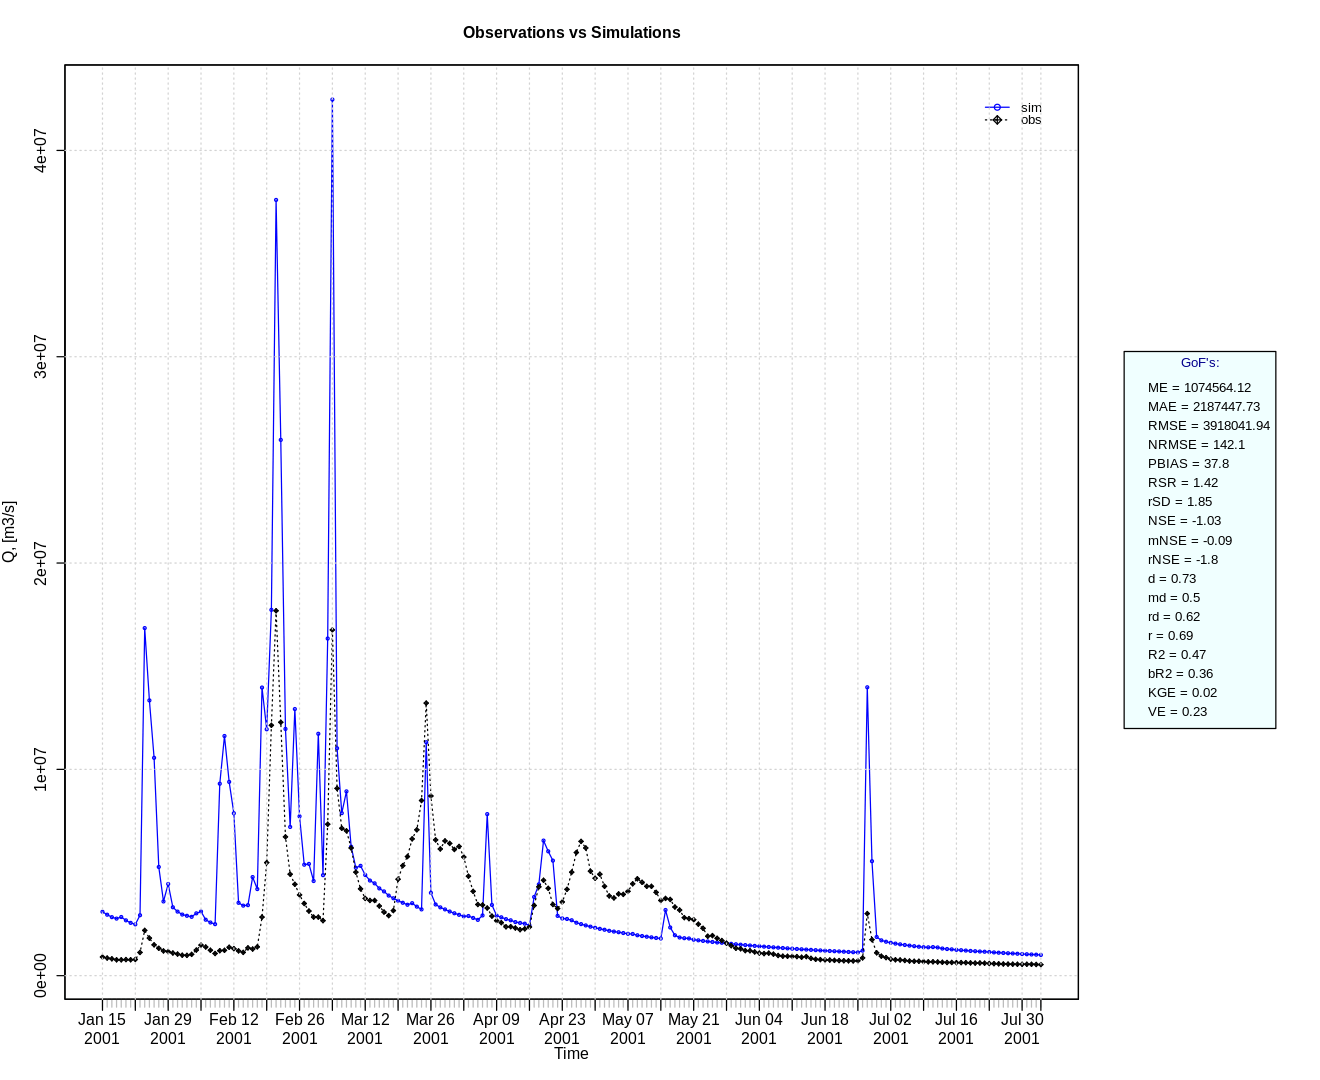
\includegraphics{Fig/fig5.png}
\caption{模拟流域径流,并与观测值比较计算模拟效果}
\end{figure}

\hypertarget{ux5730ux7406ux6570ux636eux5904ux7406}{%
\subsection*{地理数据处理}\label{ux5730ux7406ux6570ux636eux5904ux7406}}
\addcontentsline{toc}{subsection}{地理数据处理}

\begin{figure}
\centering
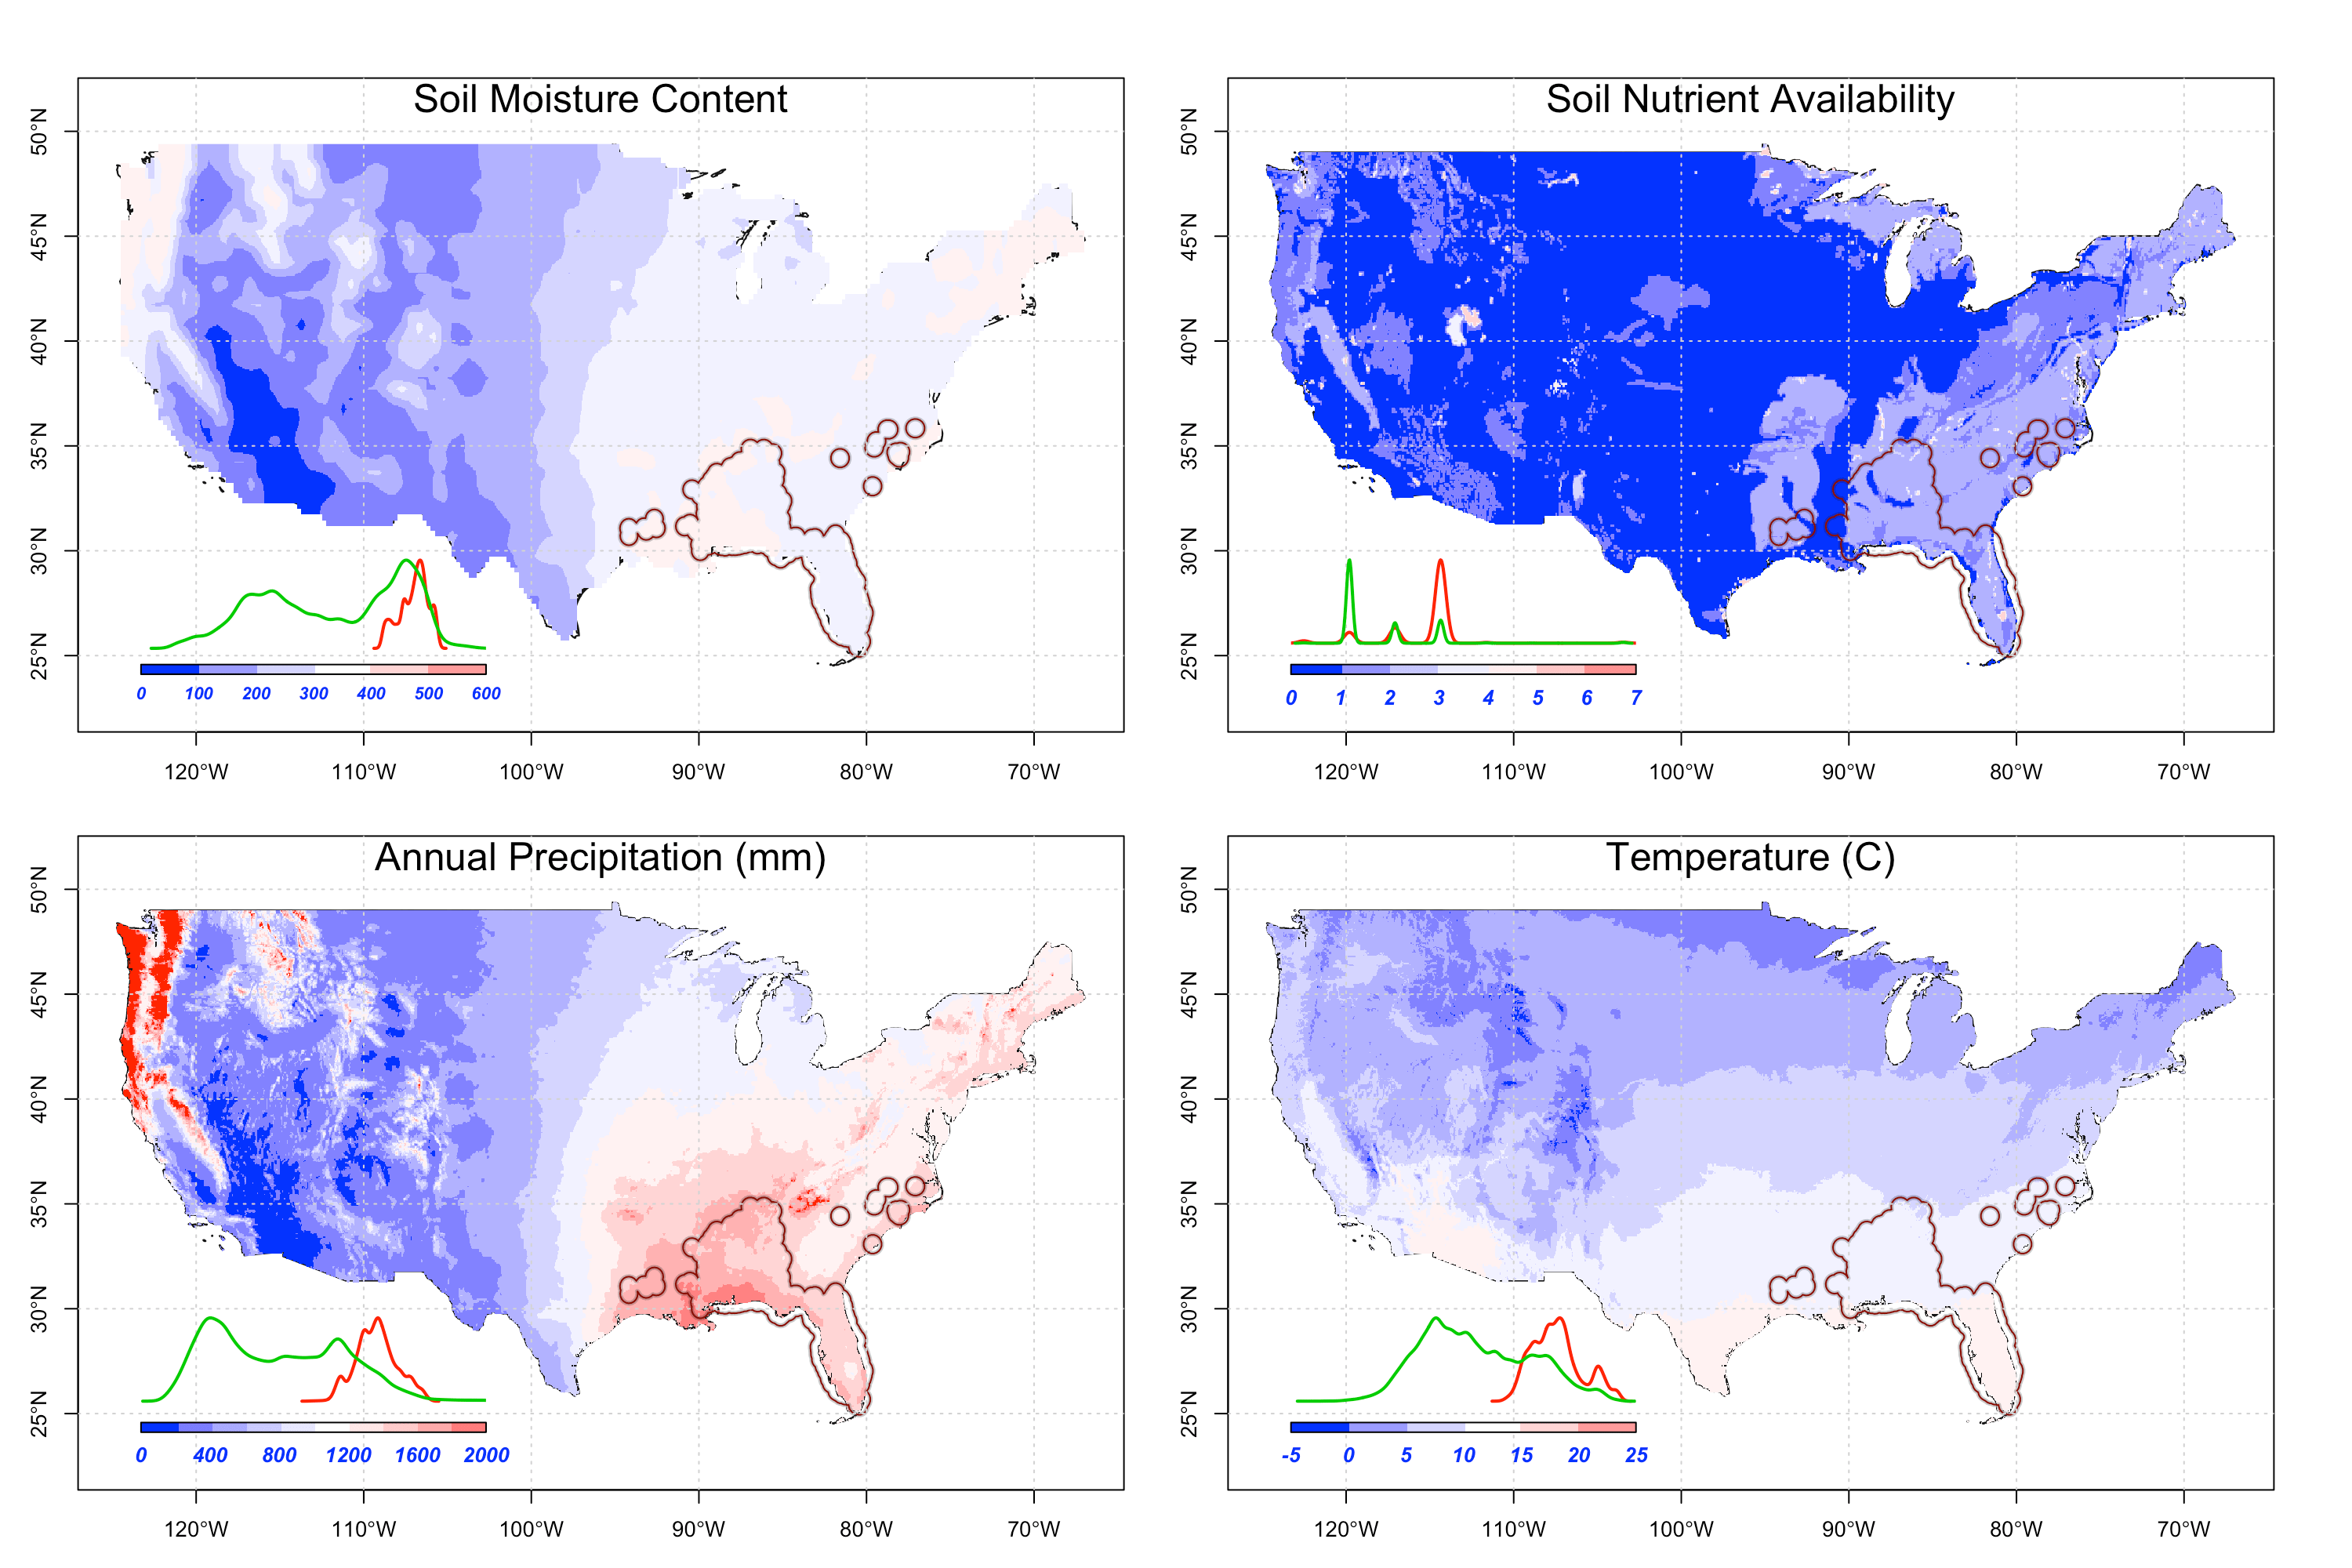
\includegraphics{Fig/fig1.png}
\caption{空间数据统计和计算}
\end{figure}

\hypertarget{ux722cux53d6ux7f51ux4e0aux516cux5f00ux6570ux636e}{%
\subsection*{爬取网上公开数据}\label{ux722cux53d6ux7f51ux4e0aux516cux5f00ux6570ux636e}}
\addcontentsline{toc}{subsection}{爬取网上公开数据}

\begin{figure}
\centering
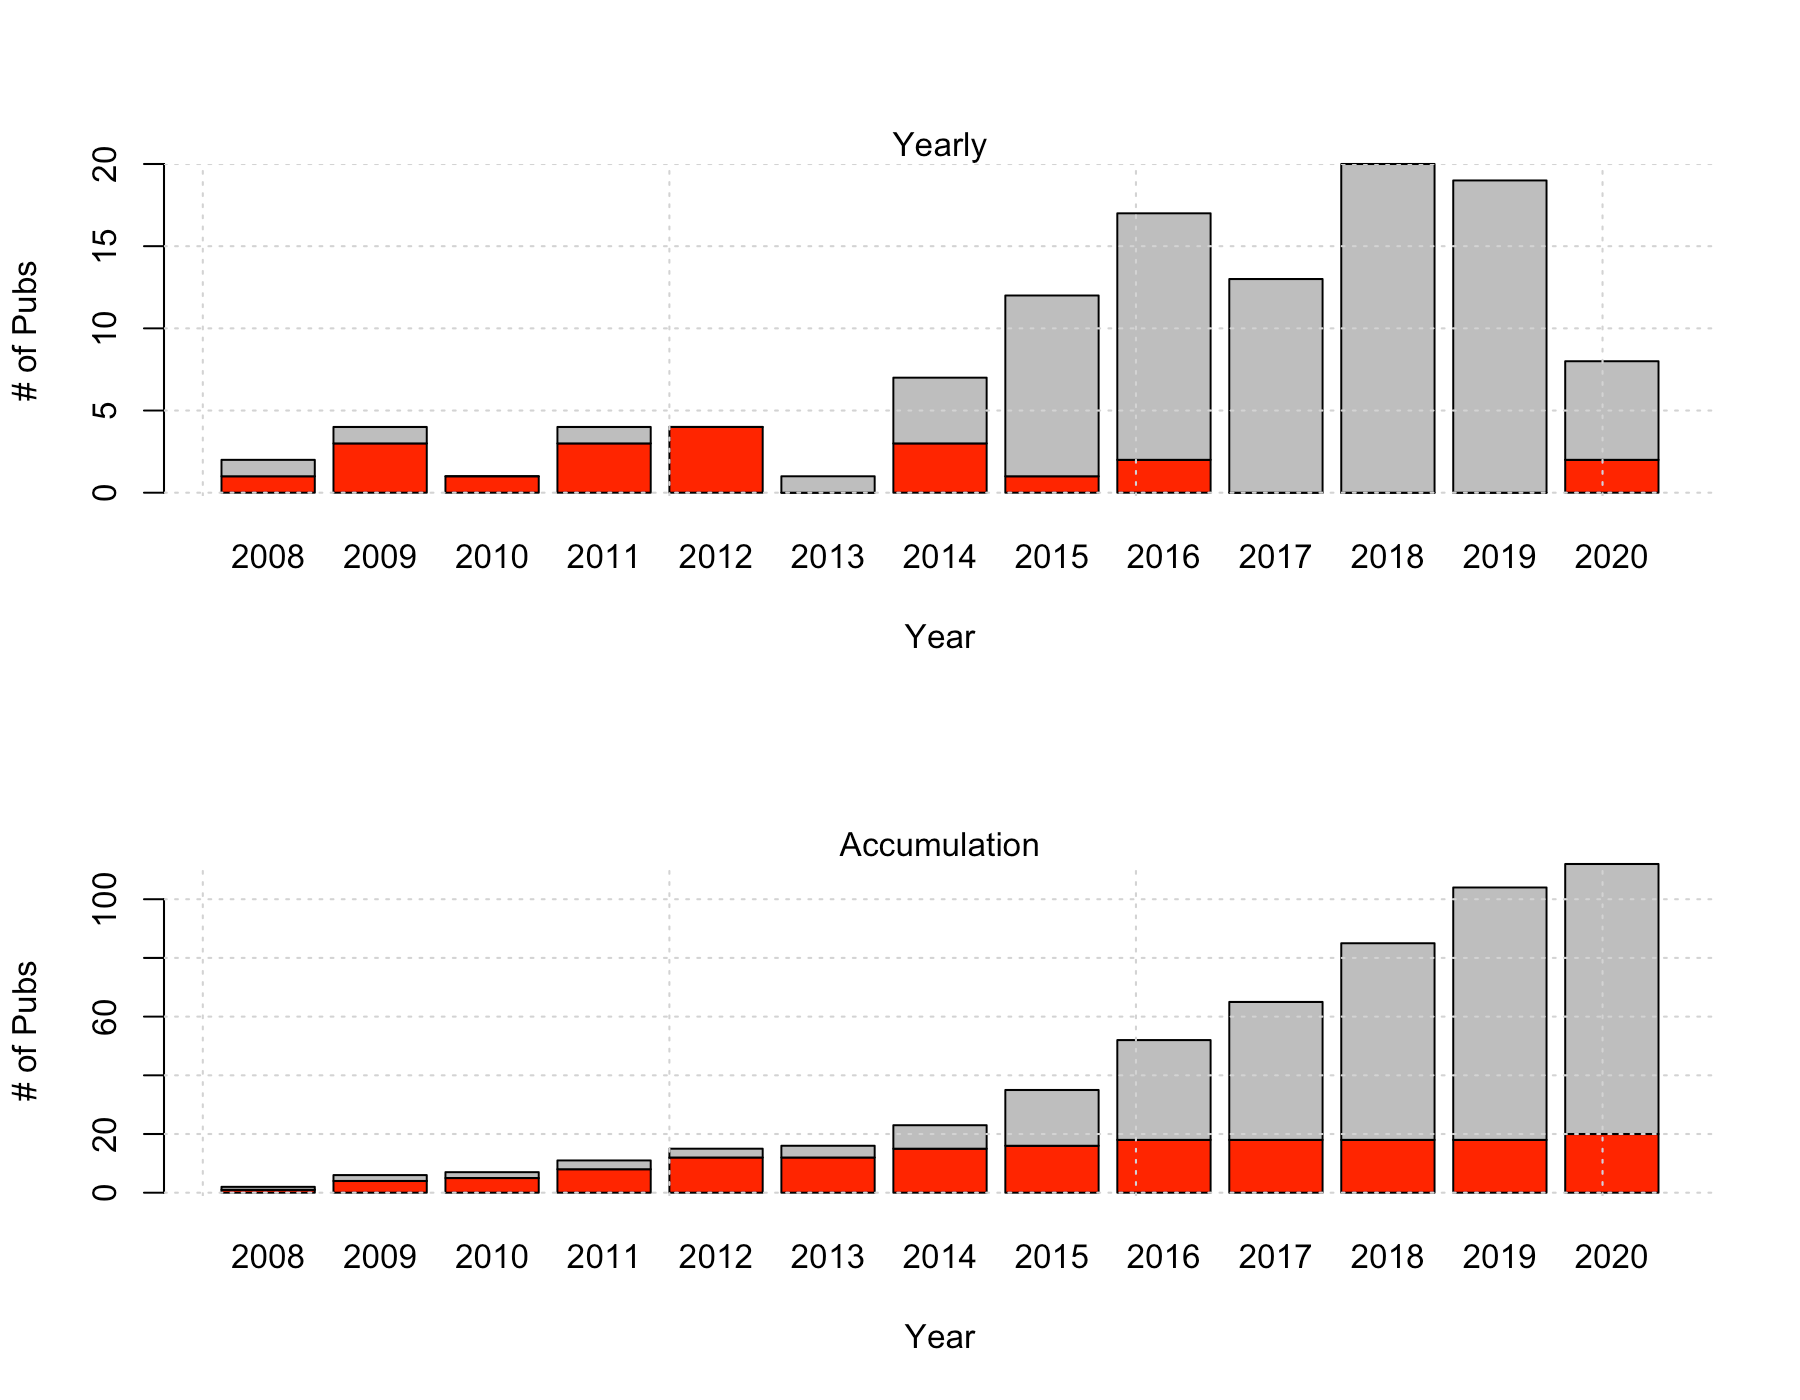
\includegraphics{Fig/fig2.png}
\caption{以上为武汉某大学的青年教授发表文章情况,12年累计数量121篇。数据来源于开放数据库Scopus}
\end{figure}

\begin{figure}
\centering
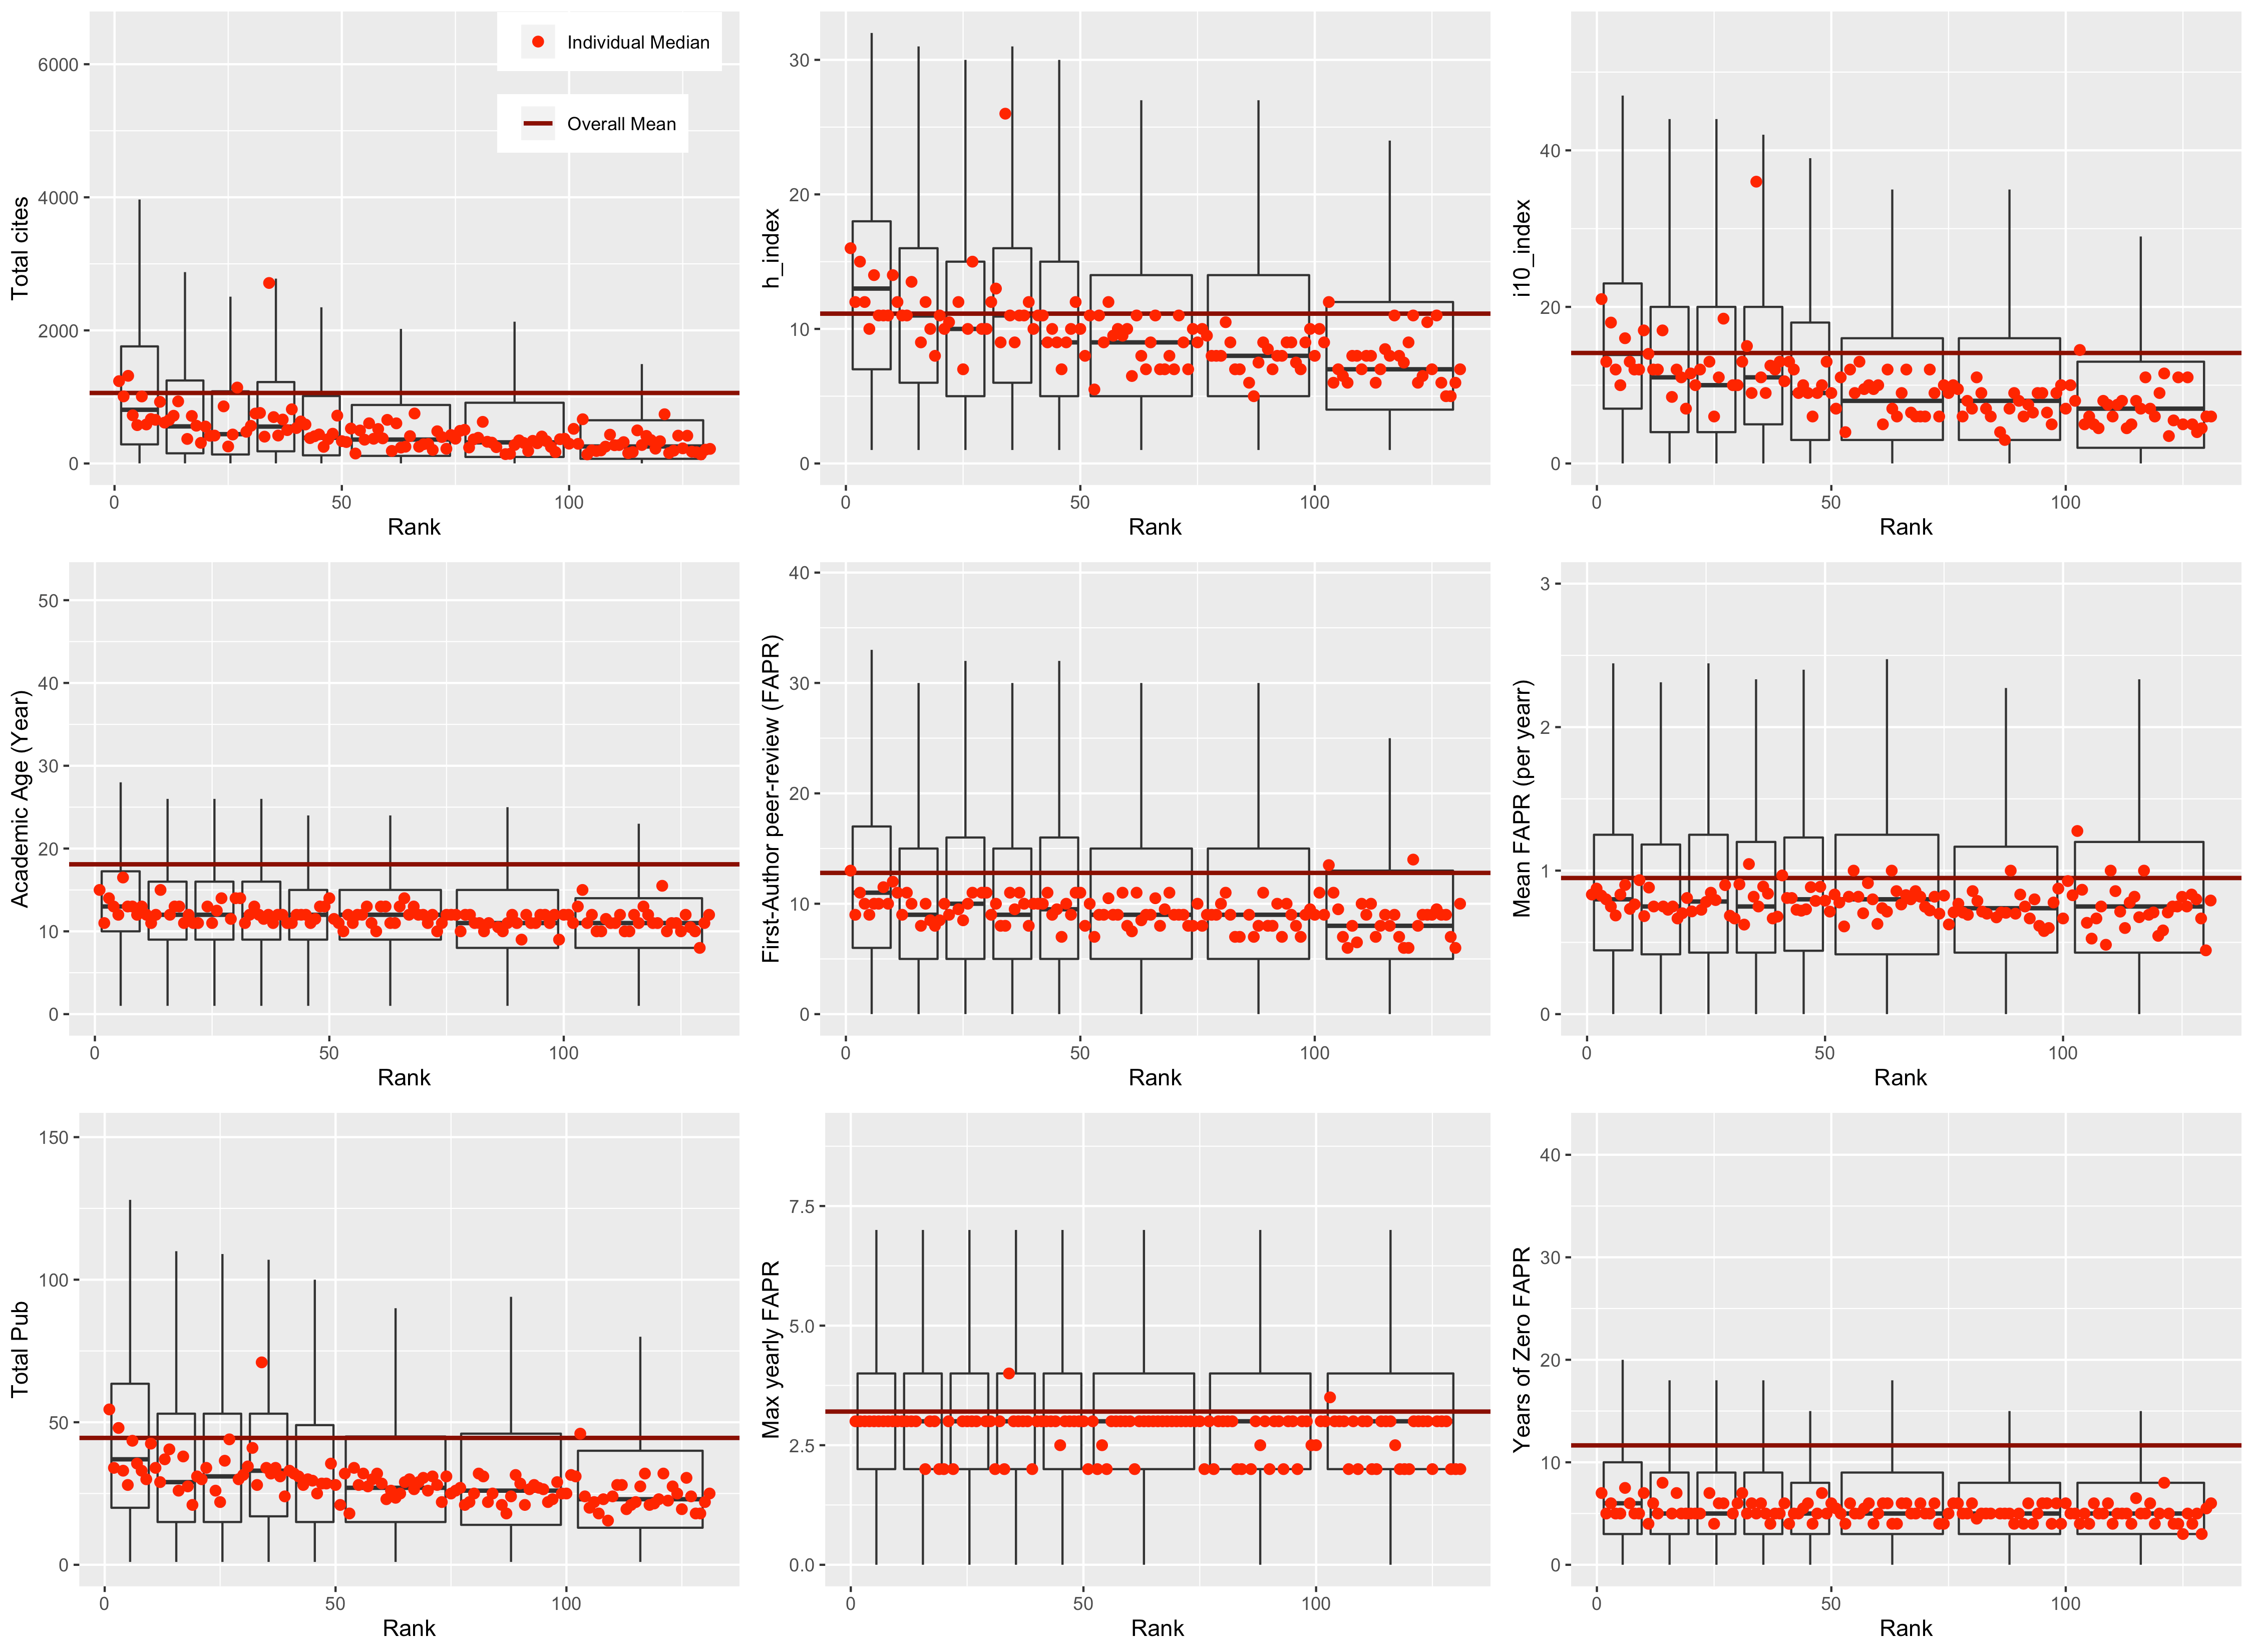
\includegraphics{Fig/fig3.png}
\caption{美国前131所大学5000+名教授文章发表情况:看平均情况,美国教授的文章数48篇,一作文章数12篇;最多产年一作数为3篇。平均数据来自于google scholar和scopus}
\end{figure}

\hypertarget{ux8ba1ux7b97ux4e0eux7ed8ux56fe}{%
\subsection*{计算与绘图}\label{ux8ba1ux7b97ux4e0eux7ed8ux56fe}}
\addcontentsline{toc}{subsection}{计算与绘图}

\begin{figure}
\centering
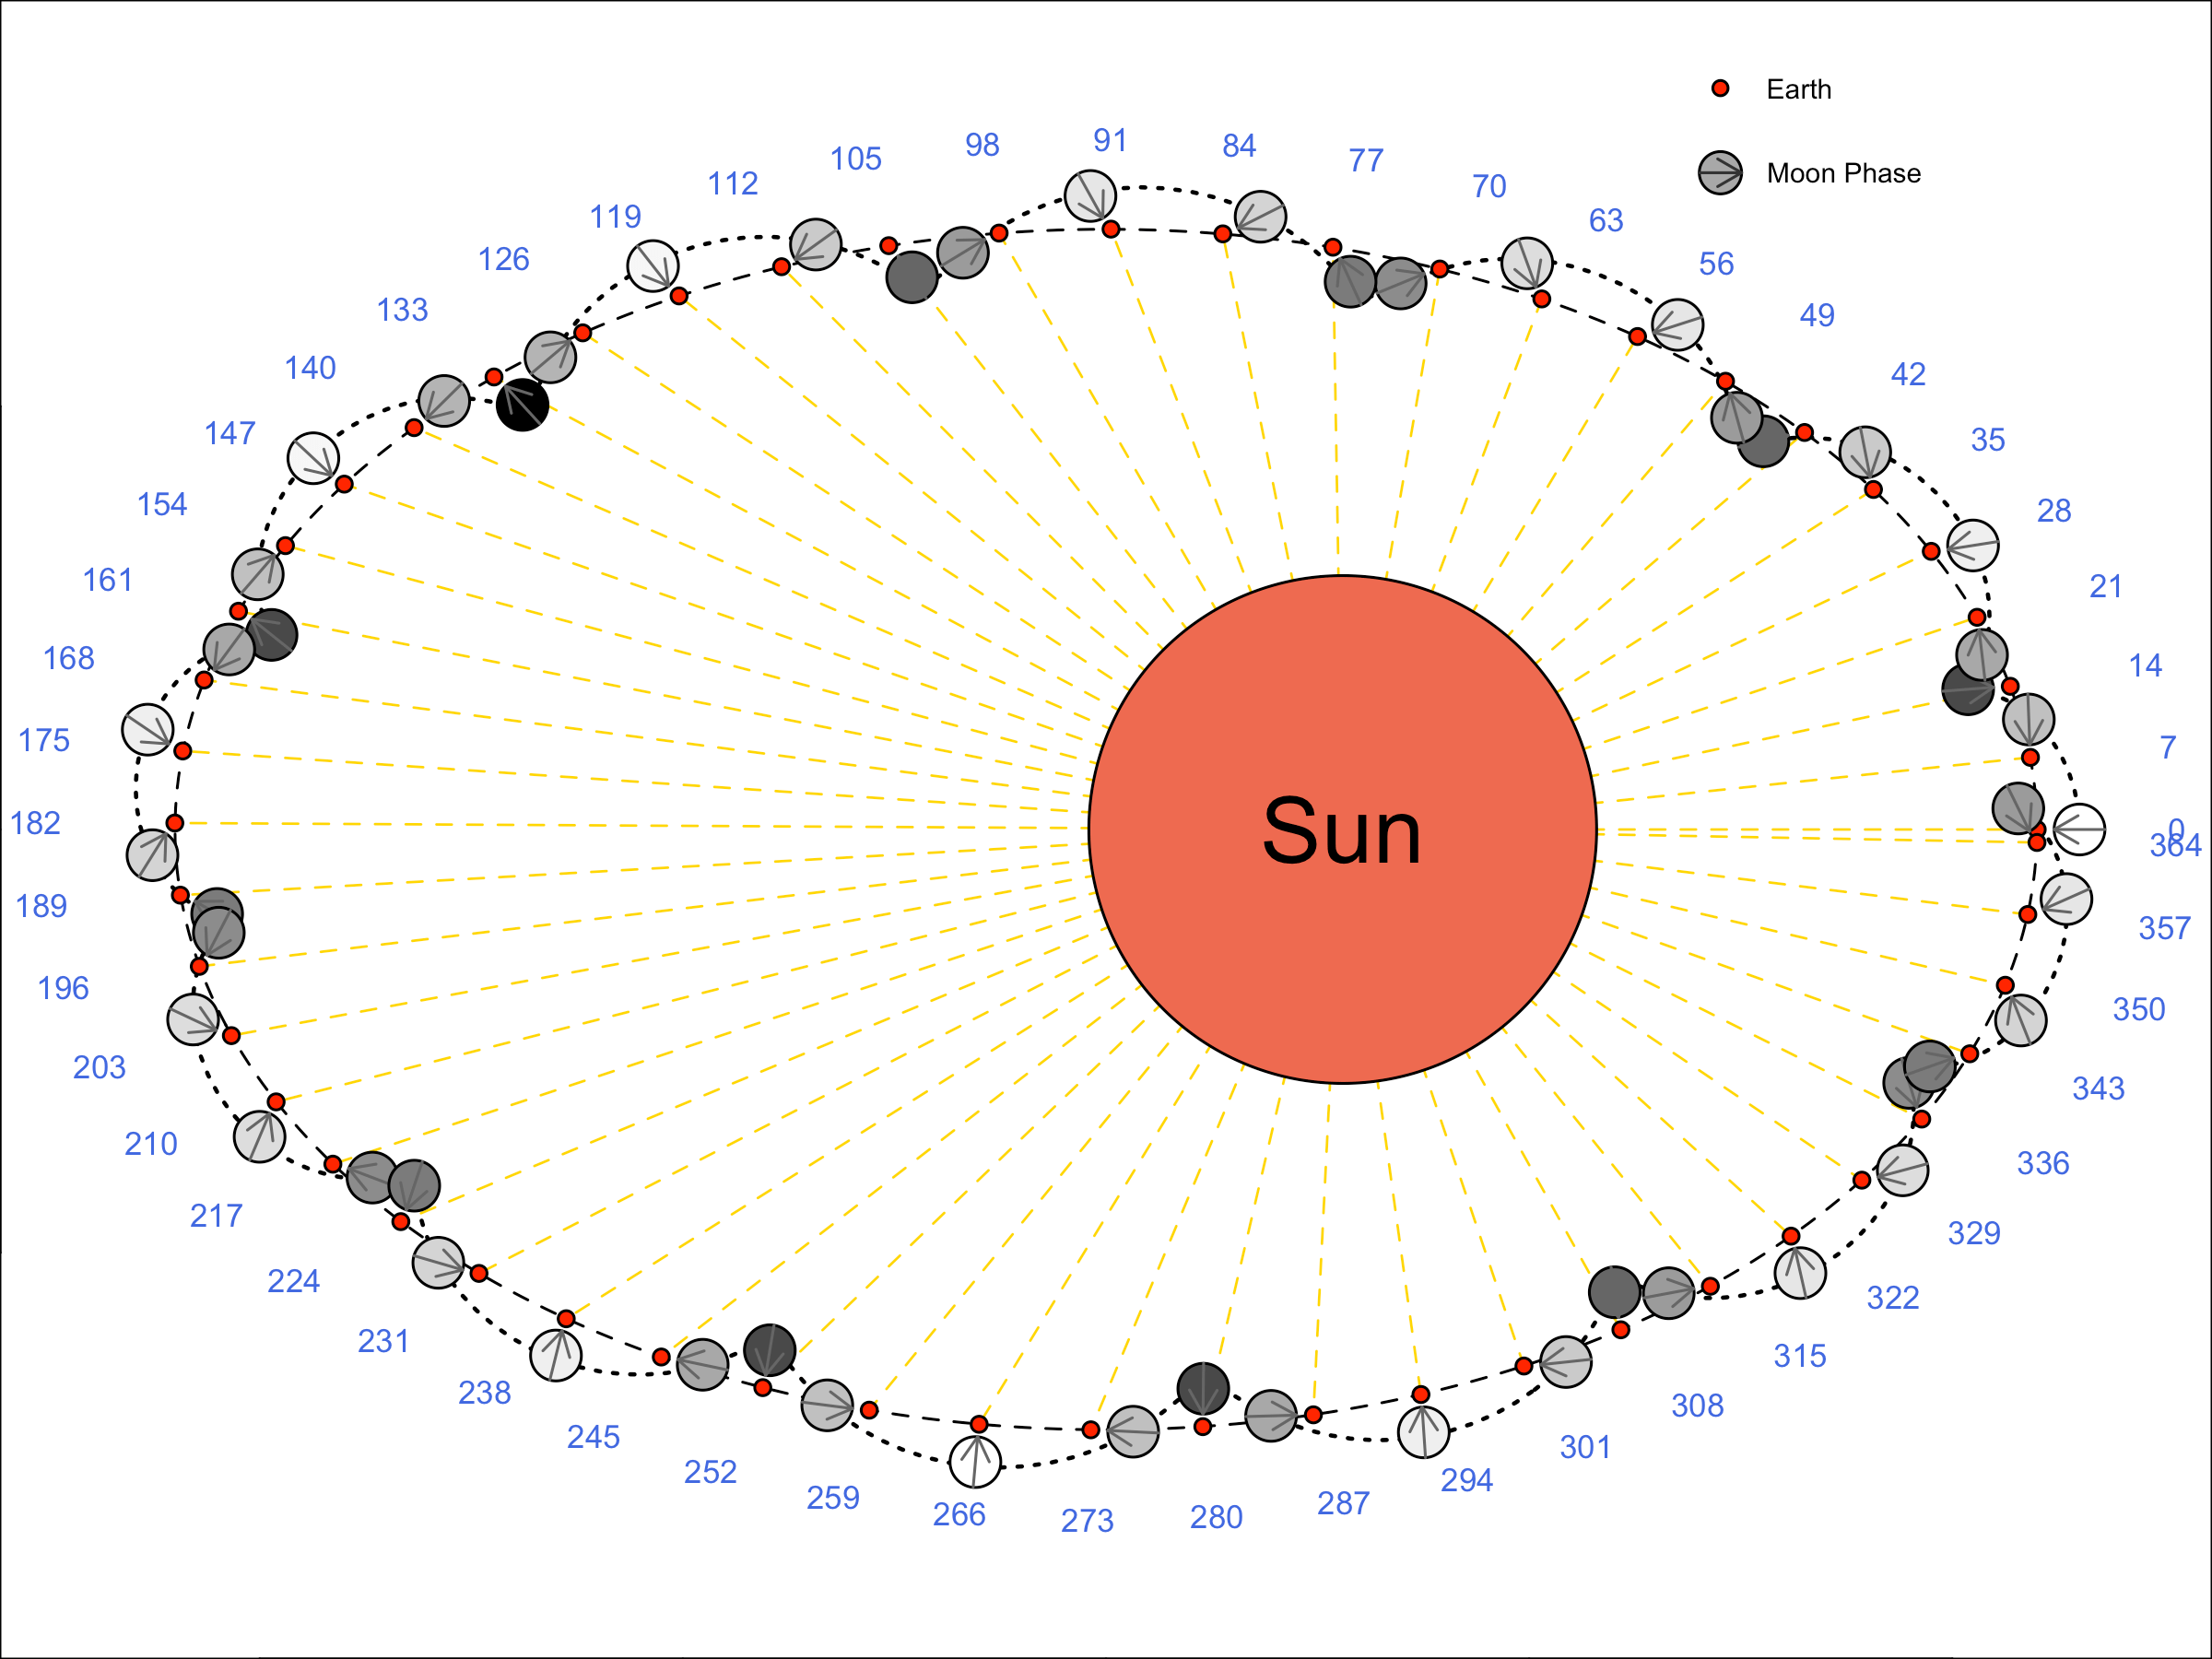
\includegraphics{Fig/fig4.png}
\caption{计算日地月关系。}
\end{figure}

\begin{figure}
\centering
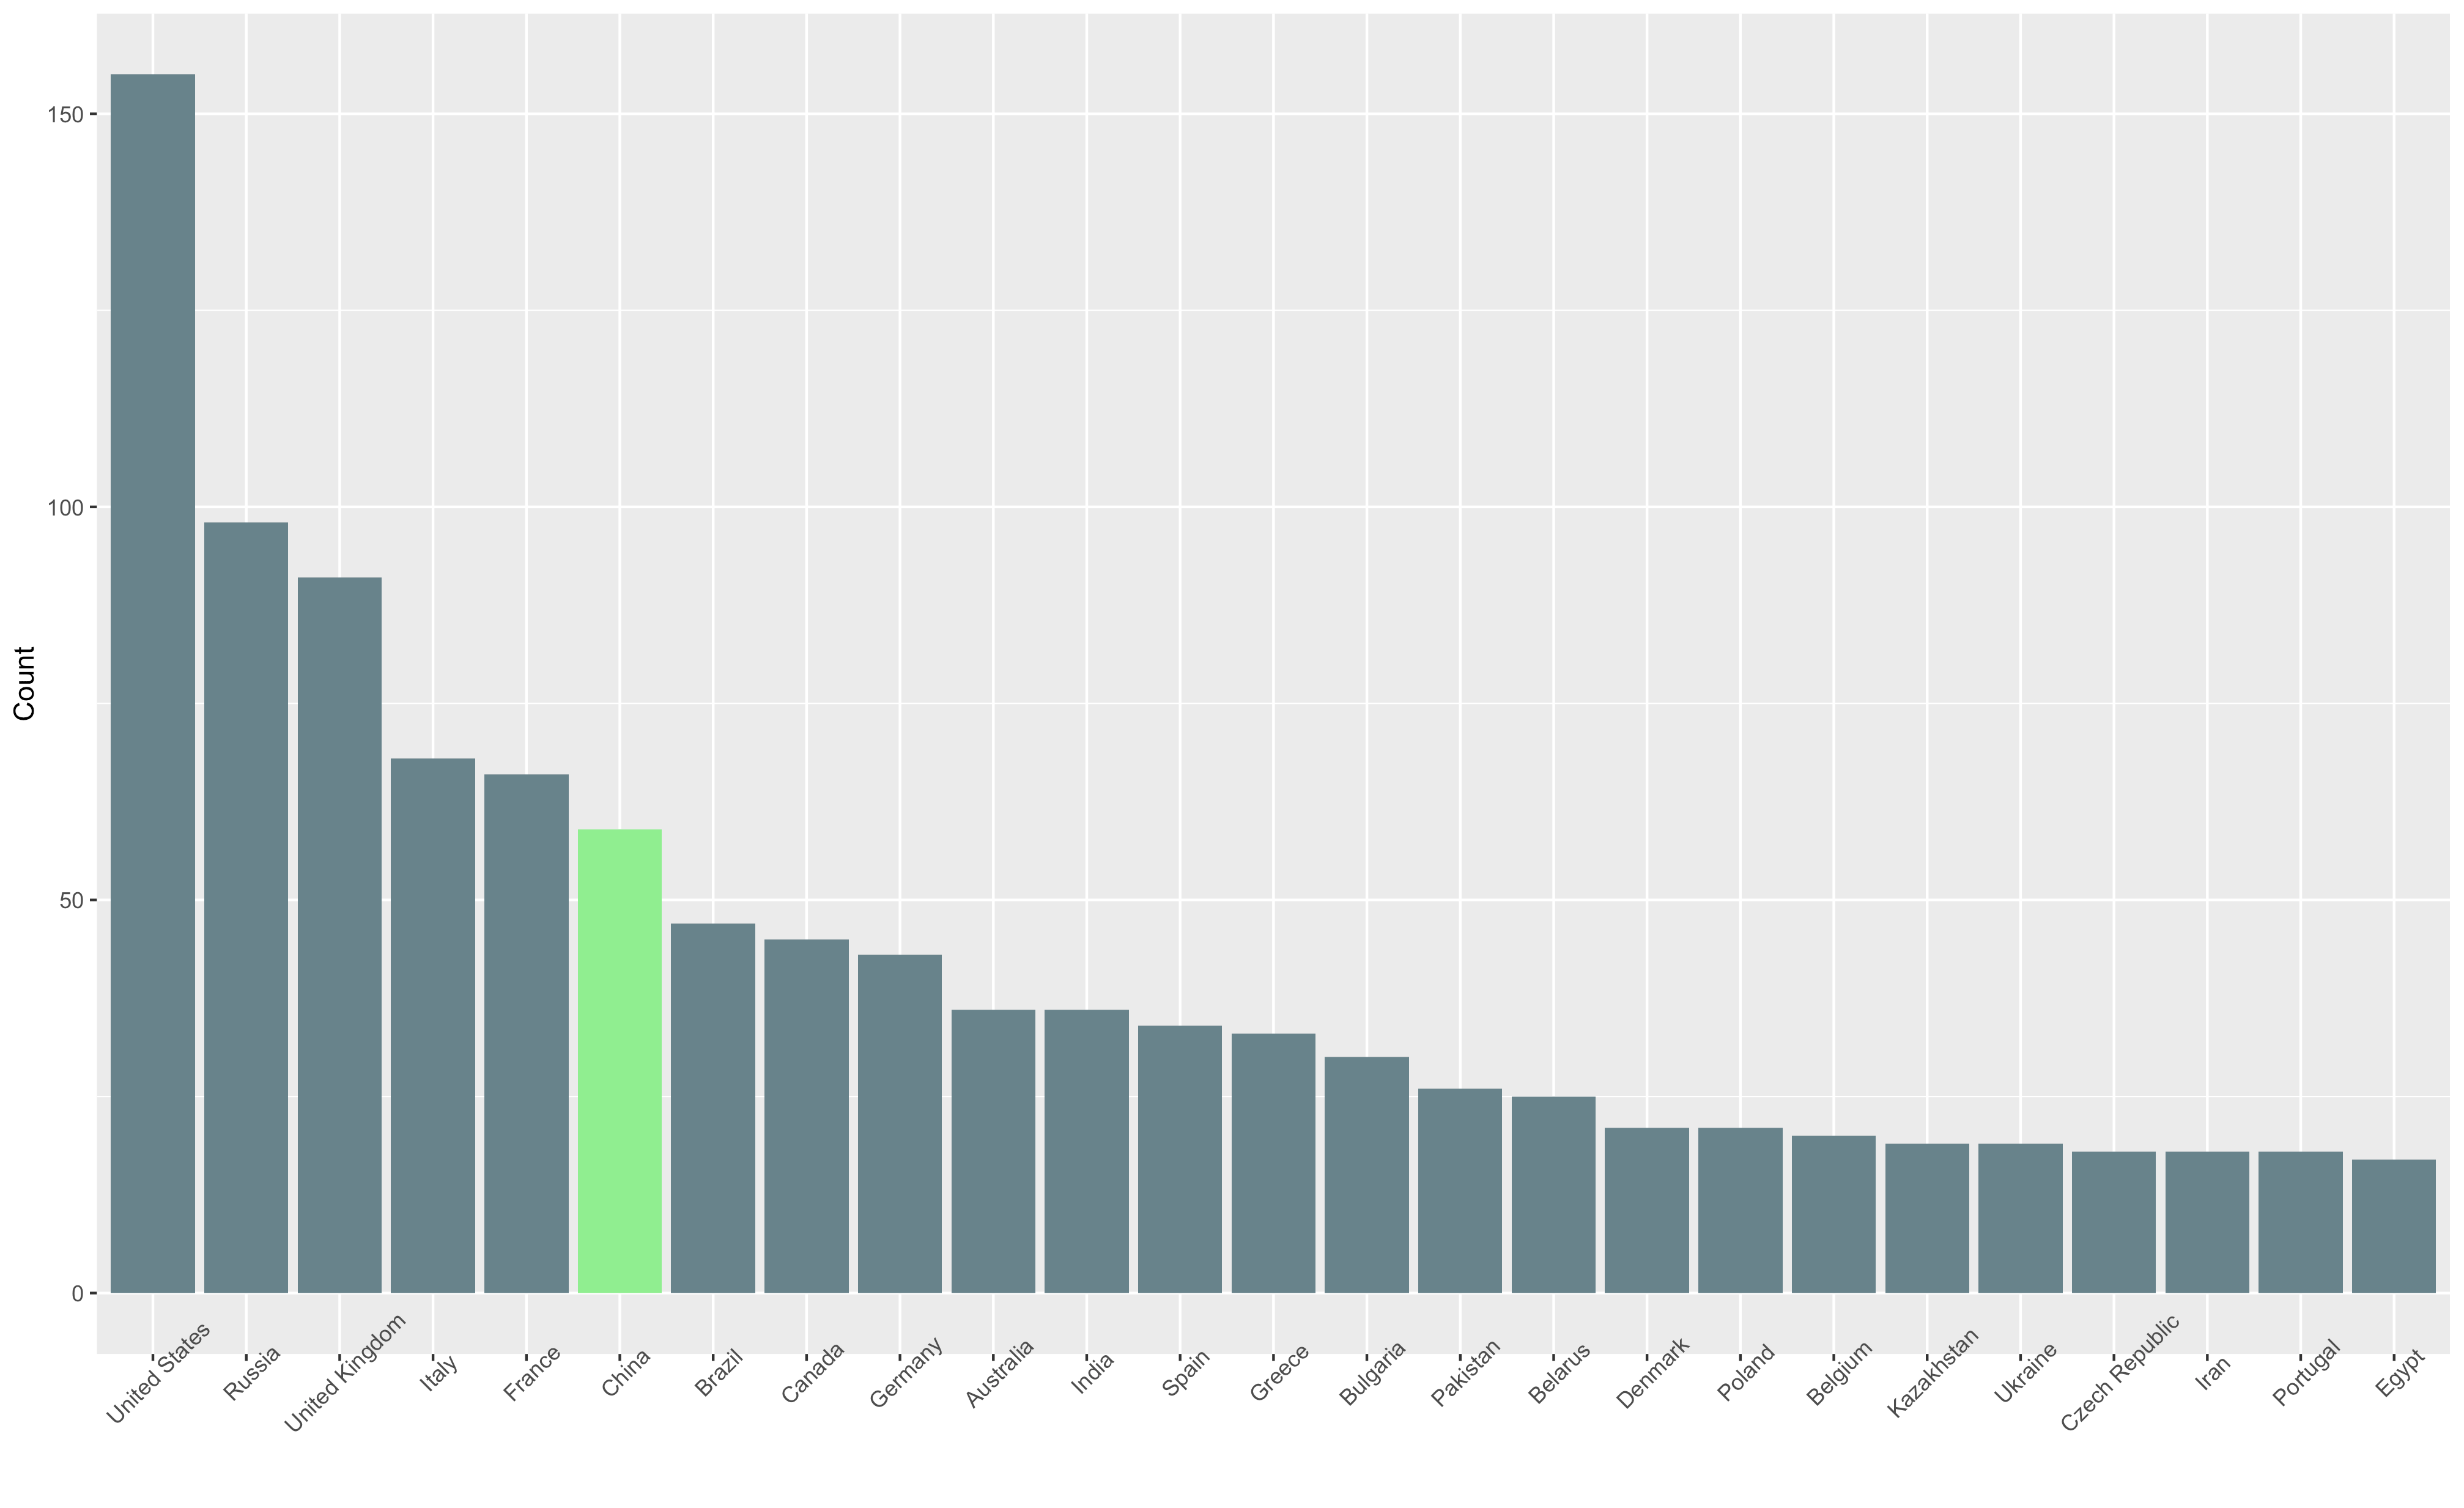
\includegraphics{Fig/fig6.png}
\caption{国际体育运动中发现服用禁药的绝对数据对比。如果应用到参与国际比赛的运动员数量或人口百分比,美欧国家排位显著靠前。}
\end{figure}

\hypertarget{ux52a8ux753bux89c6ux9891}{%
\subsection*{动画视频}\label{ux52a8ux753bux89c6ux9891}}
\addcontentsline{toc}{subsection}{动画视频}

www.shud.xyz/bookr/Movie/m1.mp4

www.shud.xyz/bookr/Movie/m2.mp4

www.shud.xyz/bookr/Movie/GRACE.mp4

www.shud.xyz/bookr/Movie/FLOOD.mp4

\hypertarget{ux5199ux4e66}{%
\subsection*{写书}\label{ux5199ux4e66}}
\addcontentsline{toc}{subsection}{写书}

Bookkdown: \url{https://bookdown.org}

\hypertarget{ux5c0fux7a0bux5e8f}{%
\subsection*{小程序}\label{ux5c0fux7a0bux5e8f}}
\addcontentsline{toc}{subsection}{小程序}

\url{https://shiny.rstudio.com/gallery/}

\hypertarget{ux6784ux5efaux4e2aux4ebaux7f51ux7ad9}{%
\subsection*{构建个人网站}\label{ux6784ux5efaux4e2aux4ebaux7f51ux7ad9}}
\addcontentsline{toc}{subsection}{构建个人网站}

\url{https://www.blogdown.org}

\url{https://bookdown.org/yihui/blogdown/}

\hypertarget{intro}{%
\chapter{R语言介绍}\label{intro}}

R是一种功能非常强大的计算机语言,最初的强项在于统计计算,而它的强大扩展能力,在大量开发包的支持下应用于各方个面。

\begin{itemize}
\tightlist
\item
  计算
\item
  可视化
\item
  三维可视化
\item
  辅助视频
\end{itemize}

\hypertarget{ux5b89ux88c5rux73afux5883}{%
\section{安装R环境}\label{ux5b89ux88c5rux73afux5883}}

R下载地址:\url{https://cran.r-project.org}。安装最新版R即可。

Rstudio下载:\url{https://rstudio.com/products/rstudio/download/}。

\hypertarget{ux5b89ux88c5rux6269ux5c55ux5305}{%
\section{安装R扩展包}\label{ux5b89ux88c5rux6269ux5c55ux5305}}

如我们需要安装以下两个扩展包:\texttt{dplyr}和\texttt{ggplot2}。

\begin{verbatim}
install.packages(c("dplyr","ggplot2", 'fields', 'reshape2'))  #绘图包

install.packages('devtools')  #用于安装正在开发中的软件包。

install.packages(c('zoo', 'xts') ) # 时间序列数据

\end{verbatim}

当需要使用rgdal处理空间数据时,需要事先安装gdal。GDAL下载地址:\url{https://gdal.org}

\begin{verbatim}
install.packages(c('rasterVis', 'rgdal', 'raster', 'sp', 'sf', 'gstat')) #空间数据处理
\end{verbatim}

\hypertarget{ux8fd0ux884cux73afux5883}{%
\section{运行环境}\label{ux8fd0ux884cux73afux5883}}

创建一个新的工作空间:

\begin{figure}
\centering
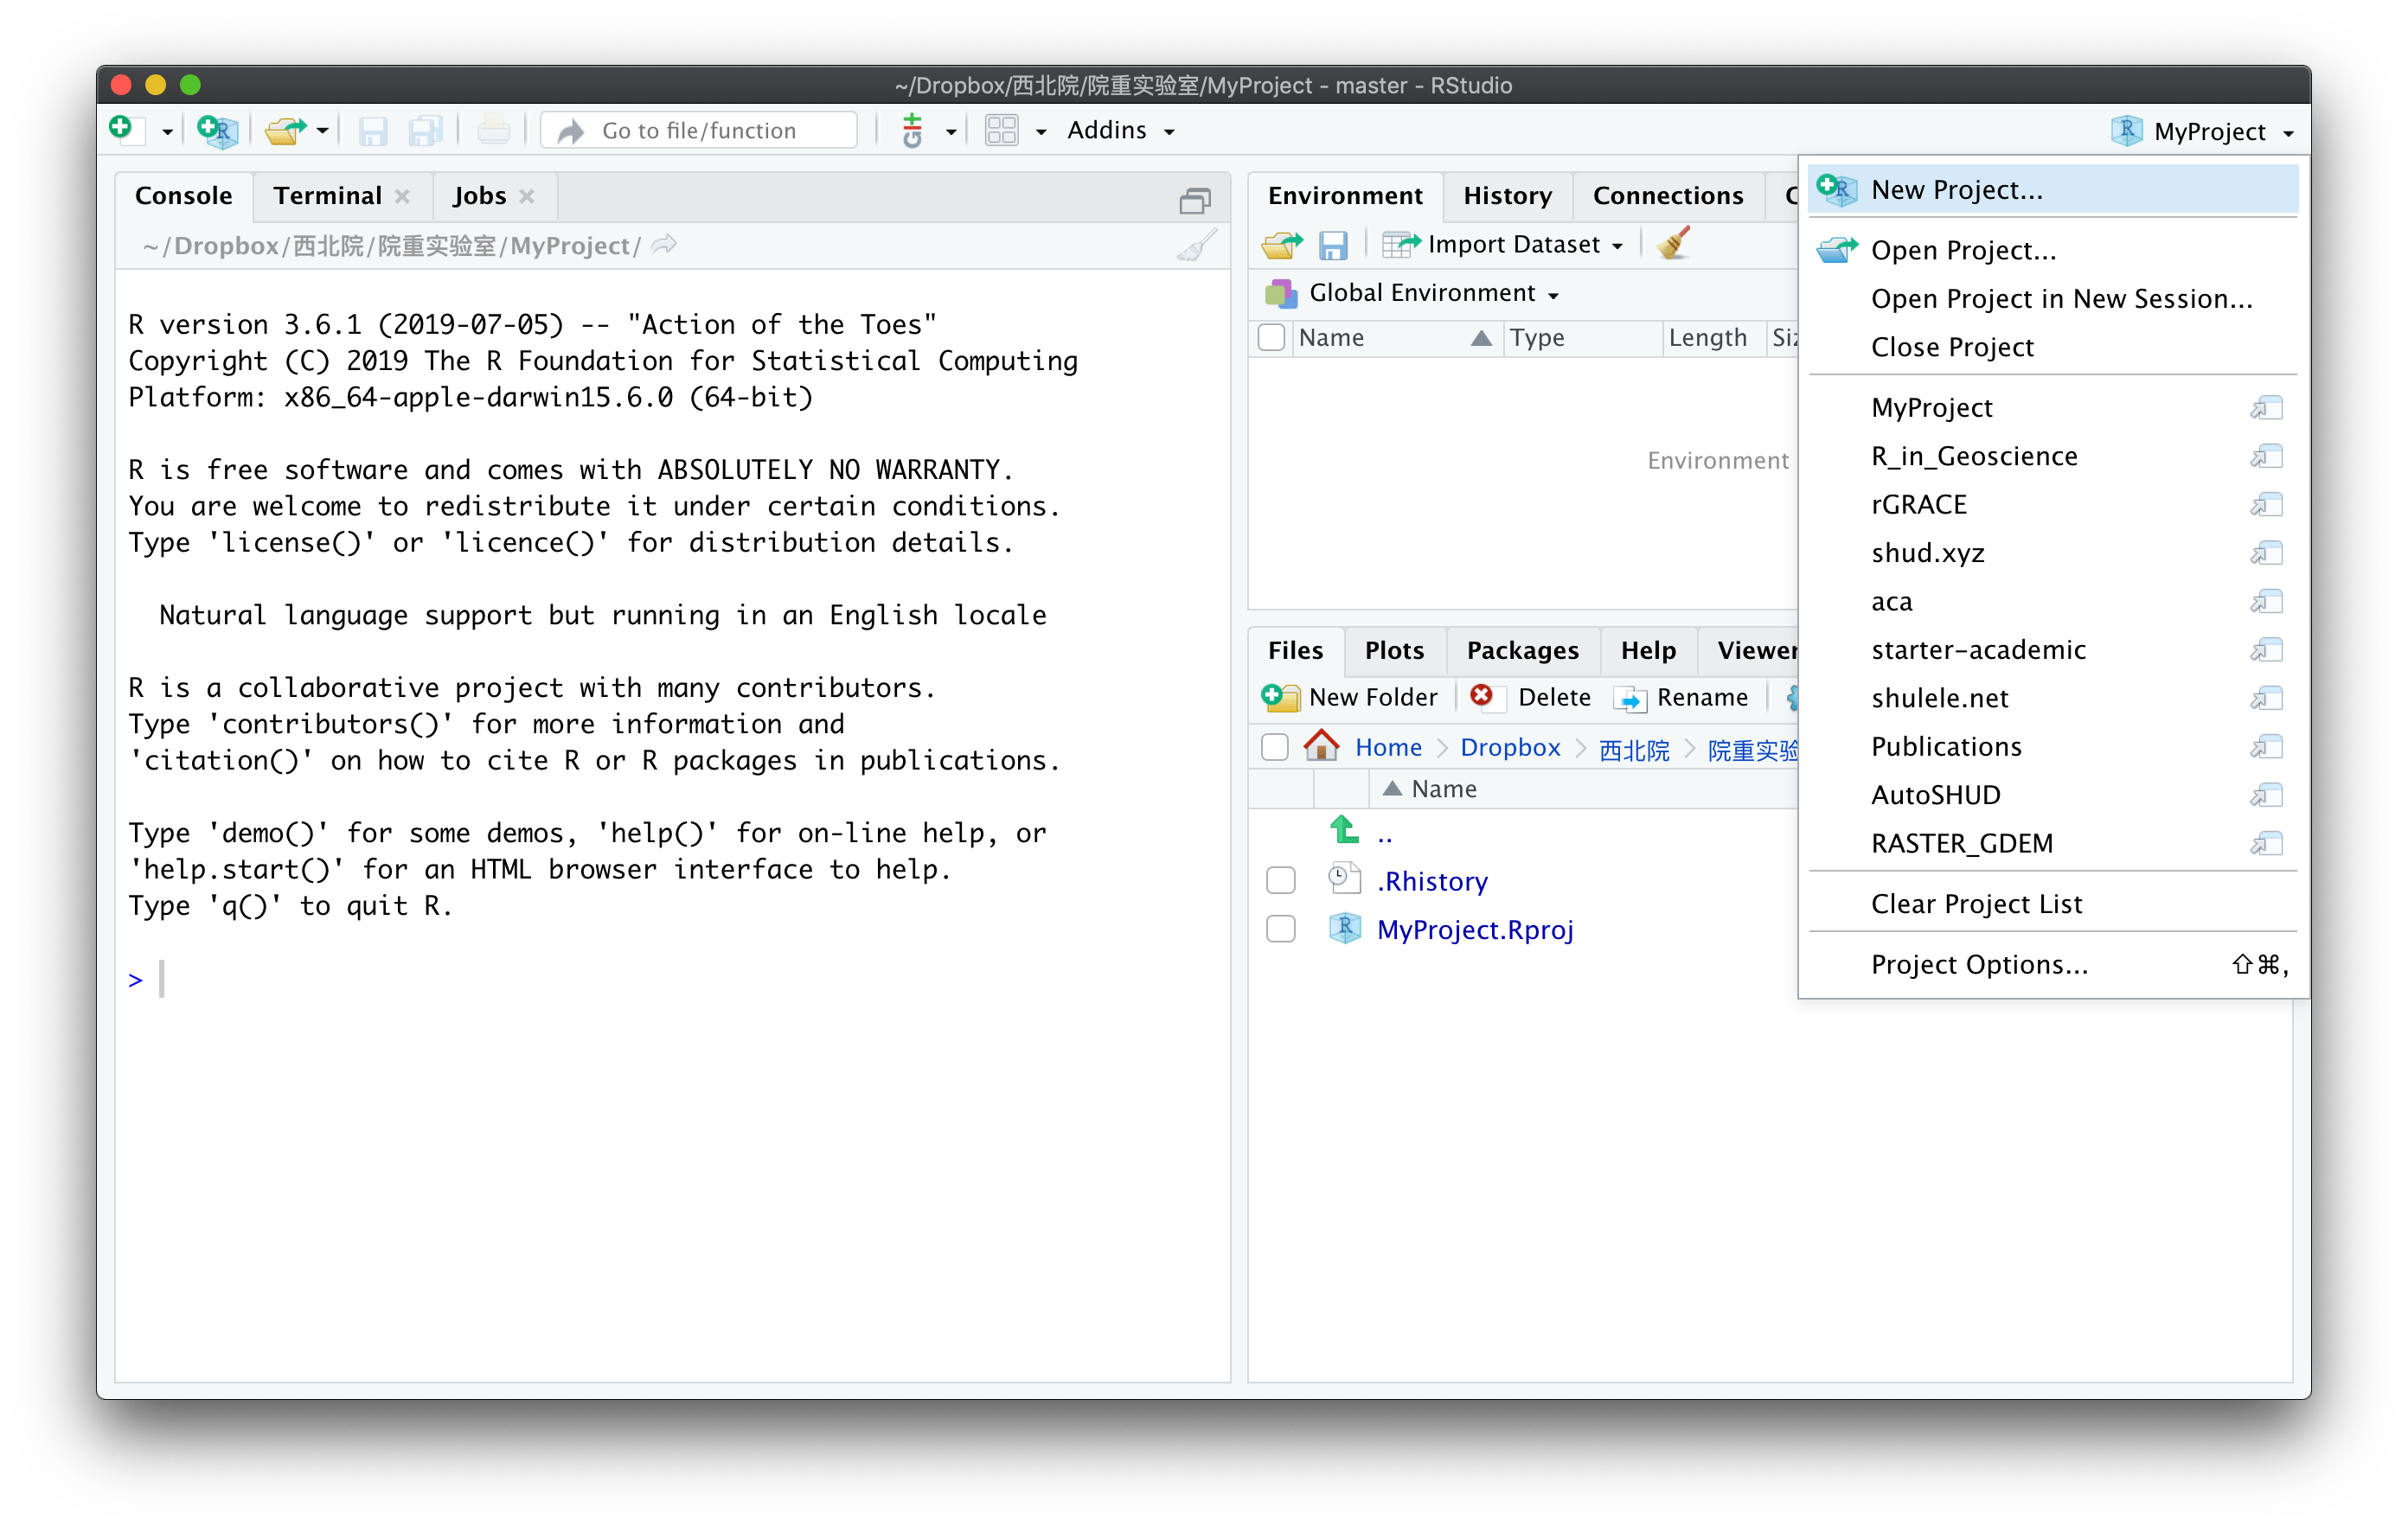
\includegraphics{Fig/ch1/Env1.png}
\caption{新建一个项目}
\end{figure}

\begin{figure}
\centering
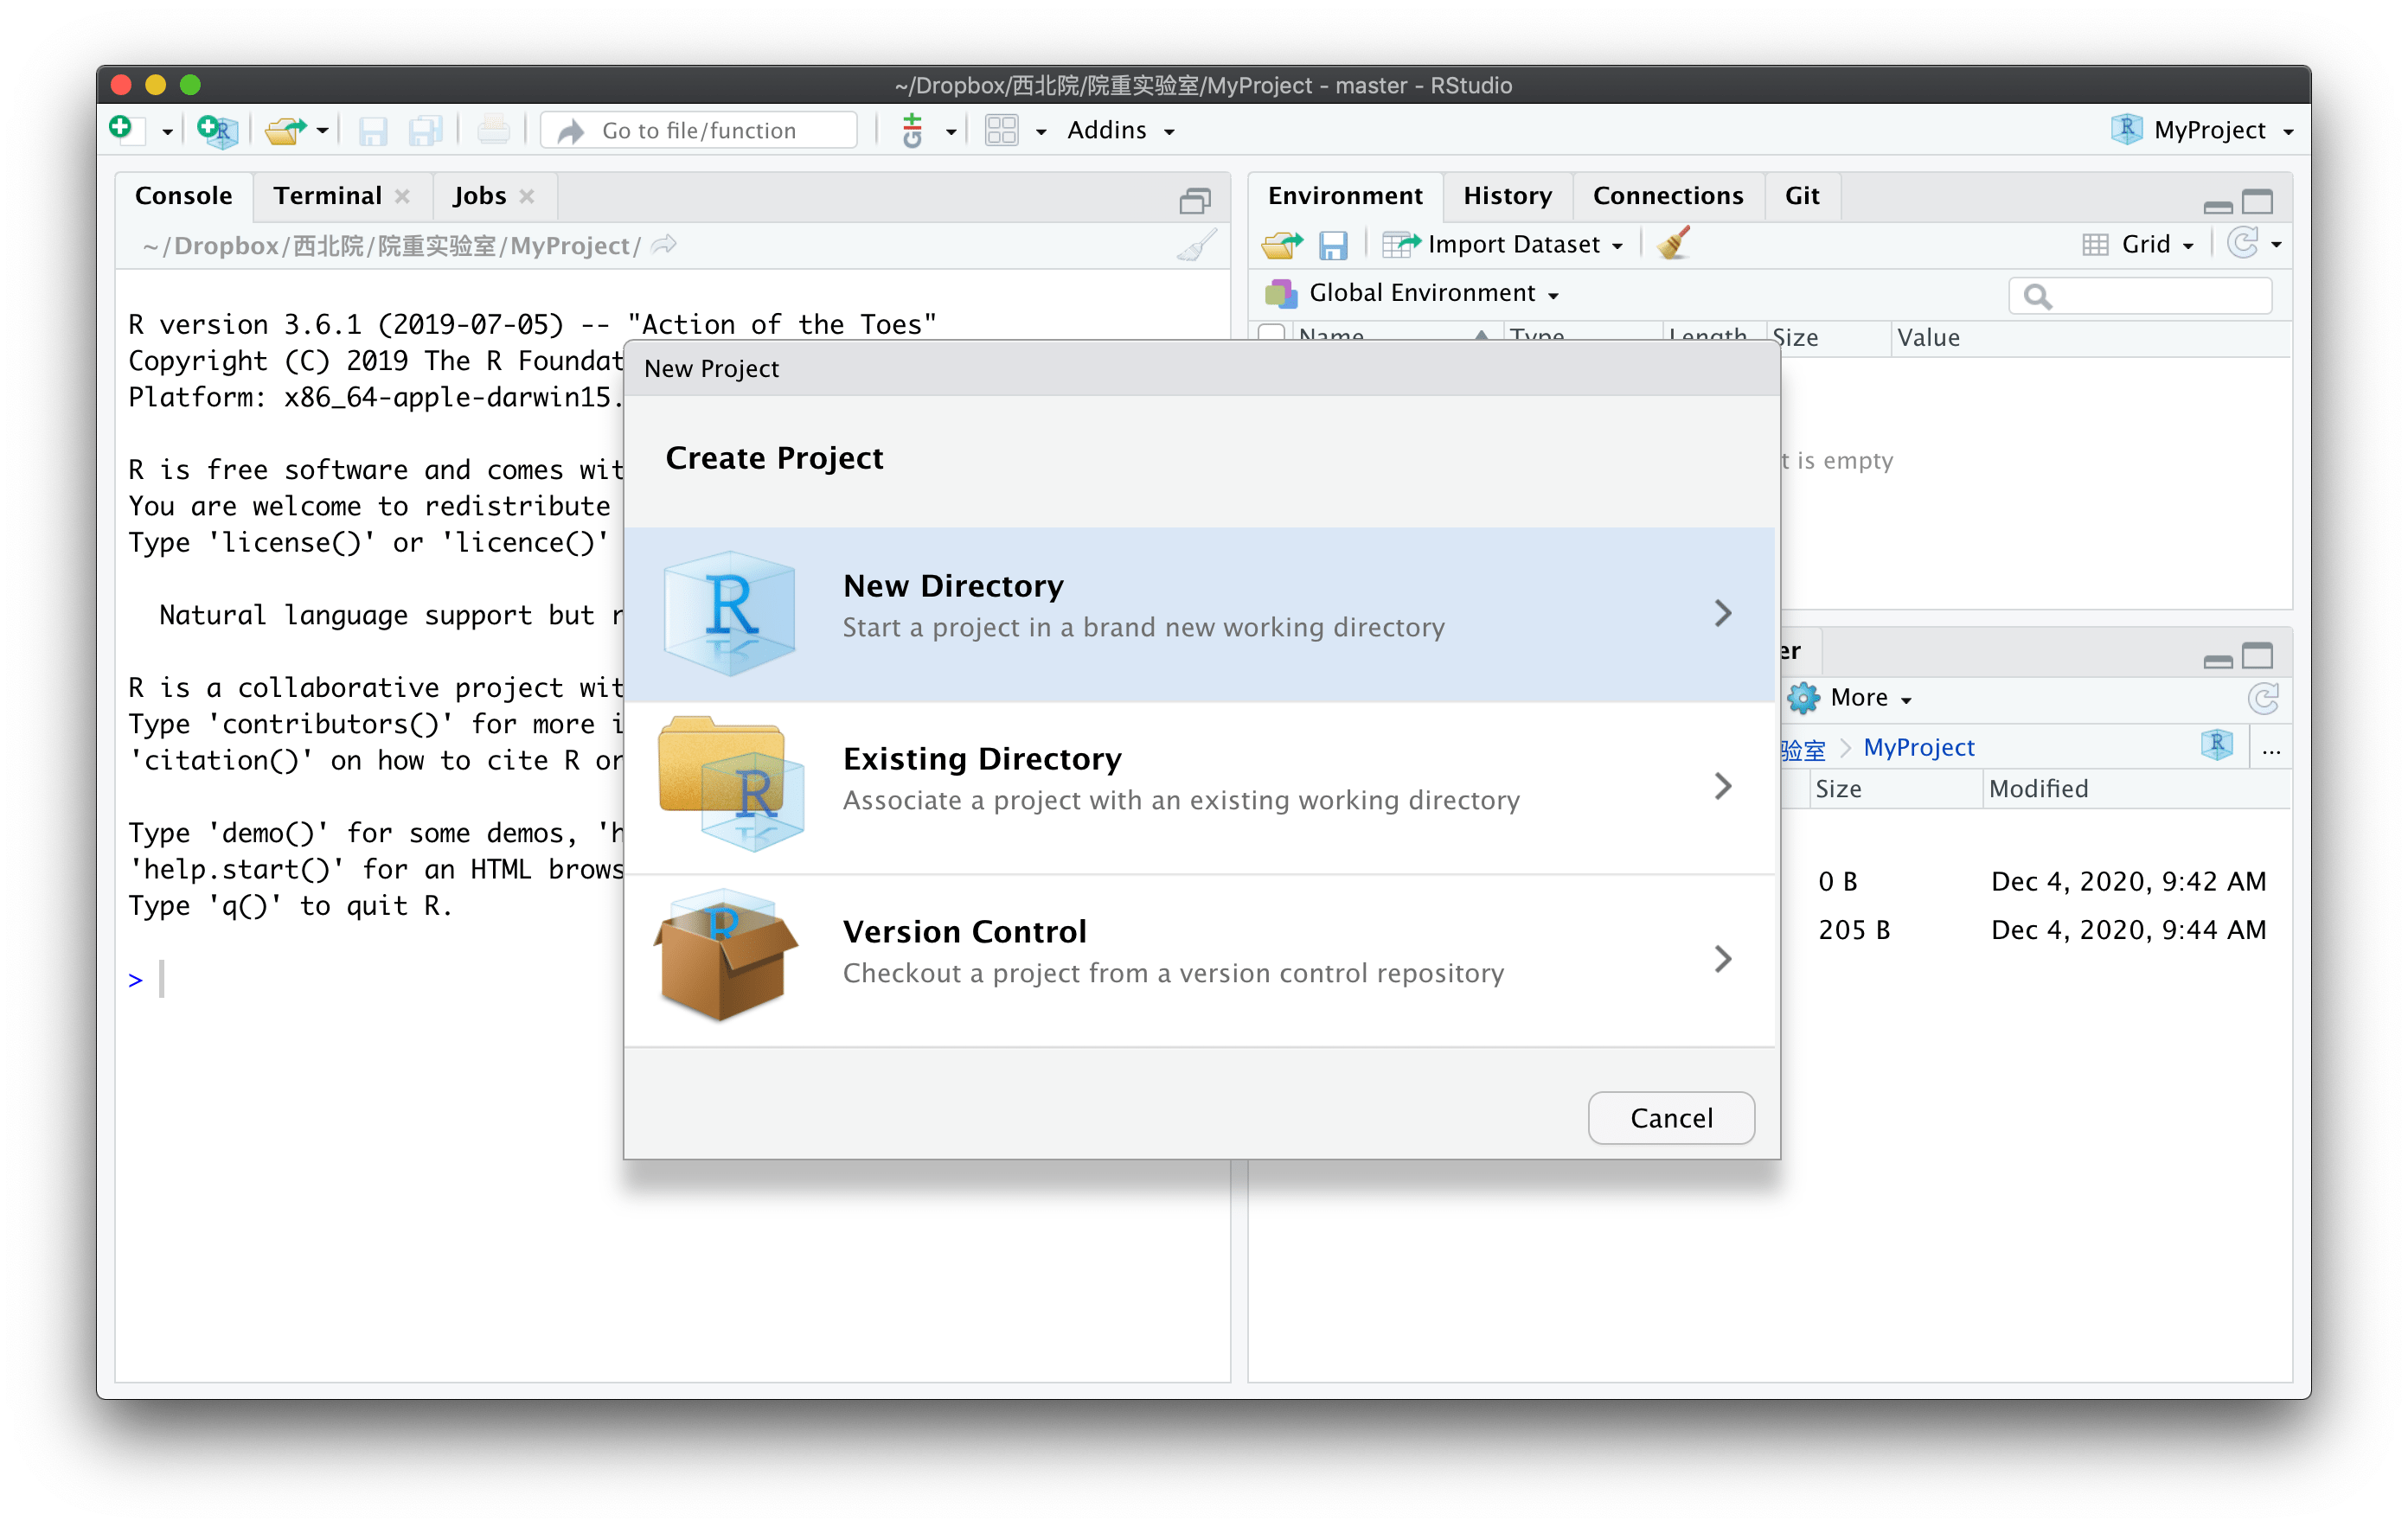
\includegraphics{Fig/ch1/Env2.png}
\caption{选择新文件夹}
\end{figure}

\begin{figure}
\centering
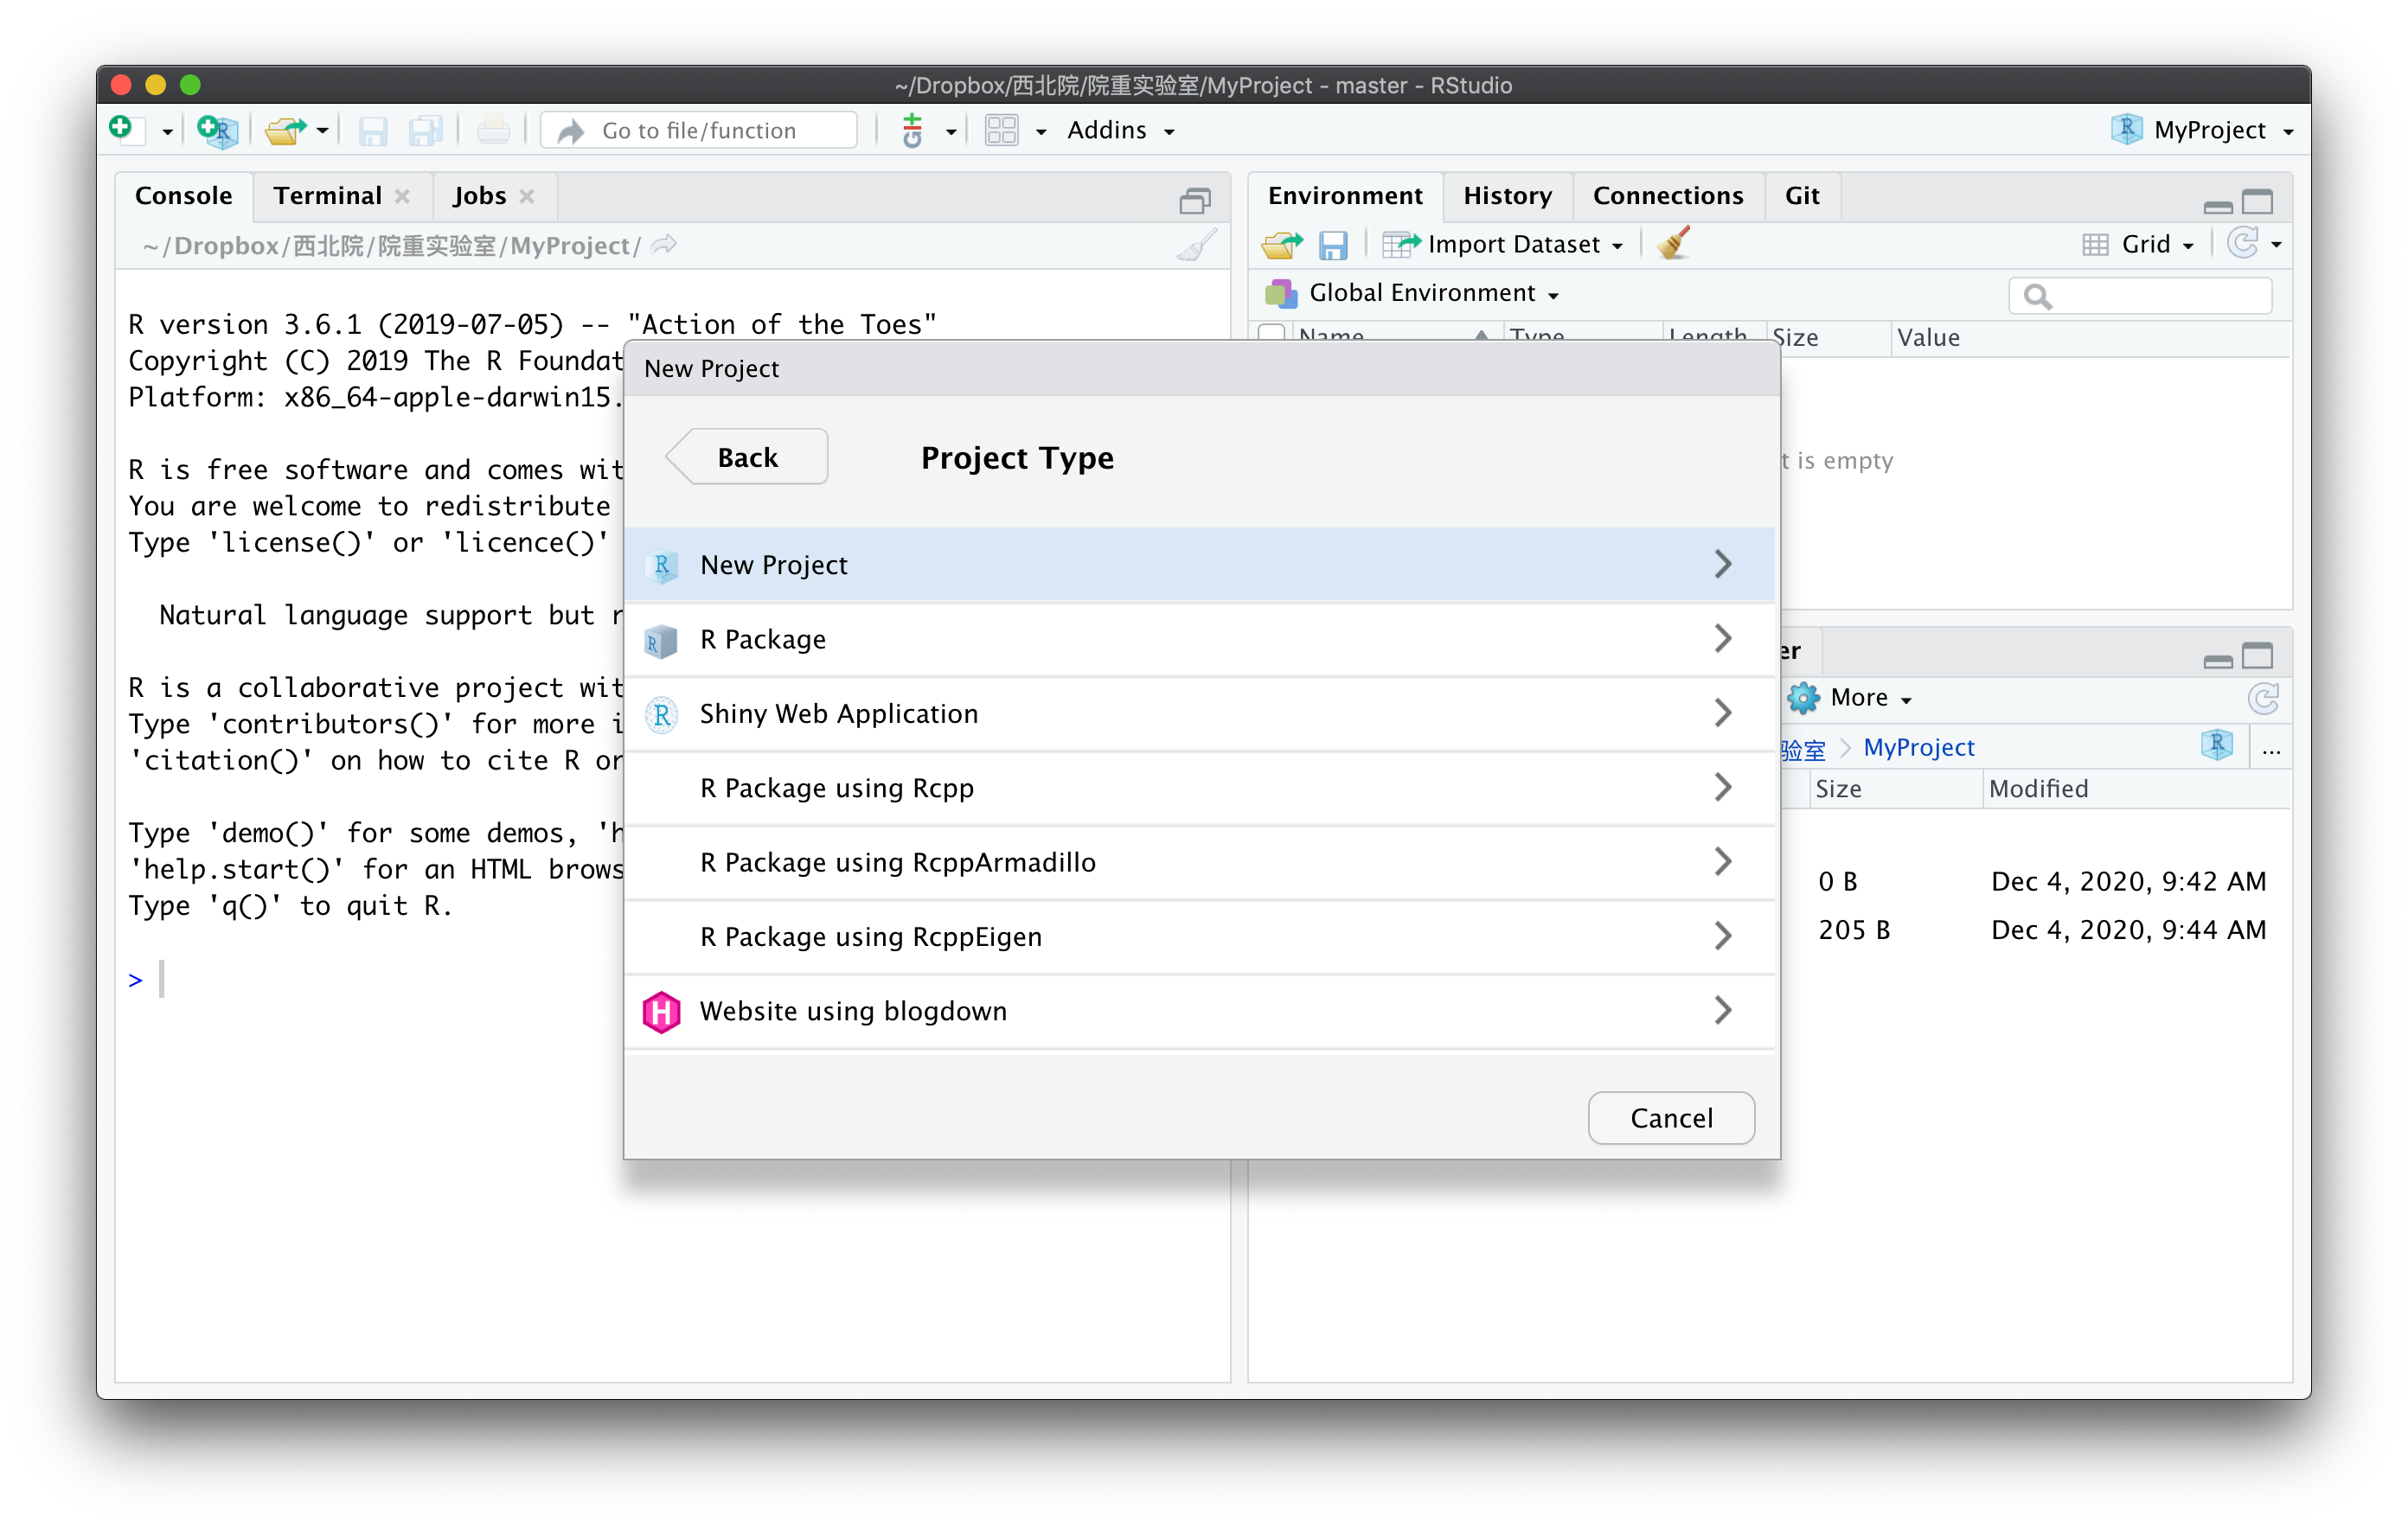
\includegraphics{Fig/ch1/Env3.png}
\caption{创建一个项目}
\end{figure}

\begin{figure}
\centering
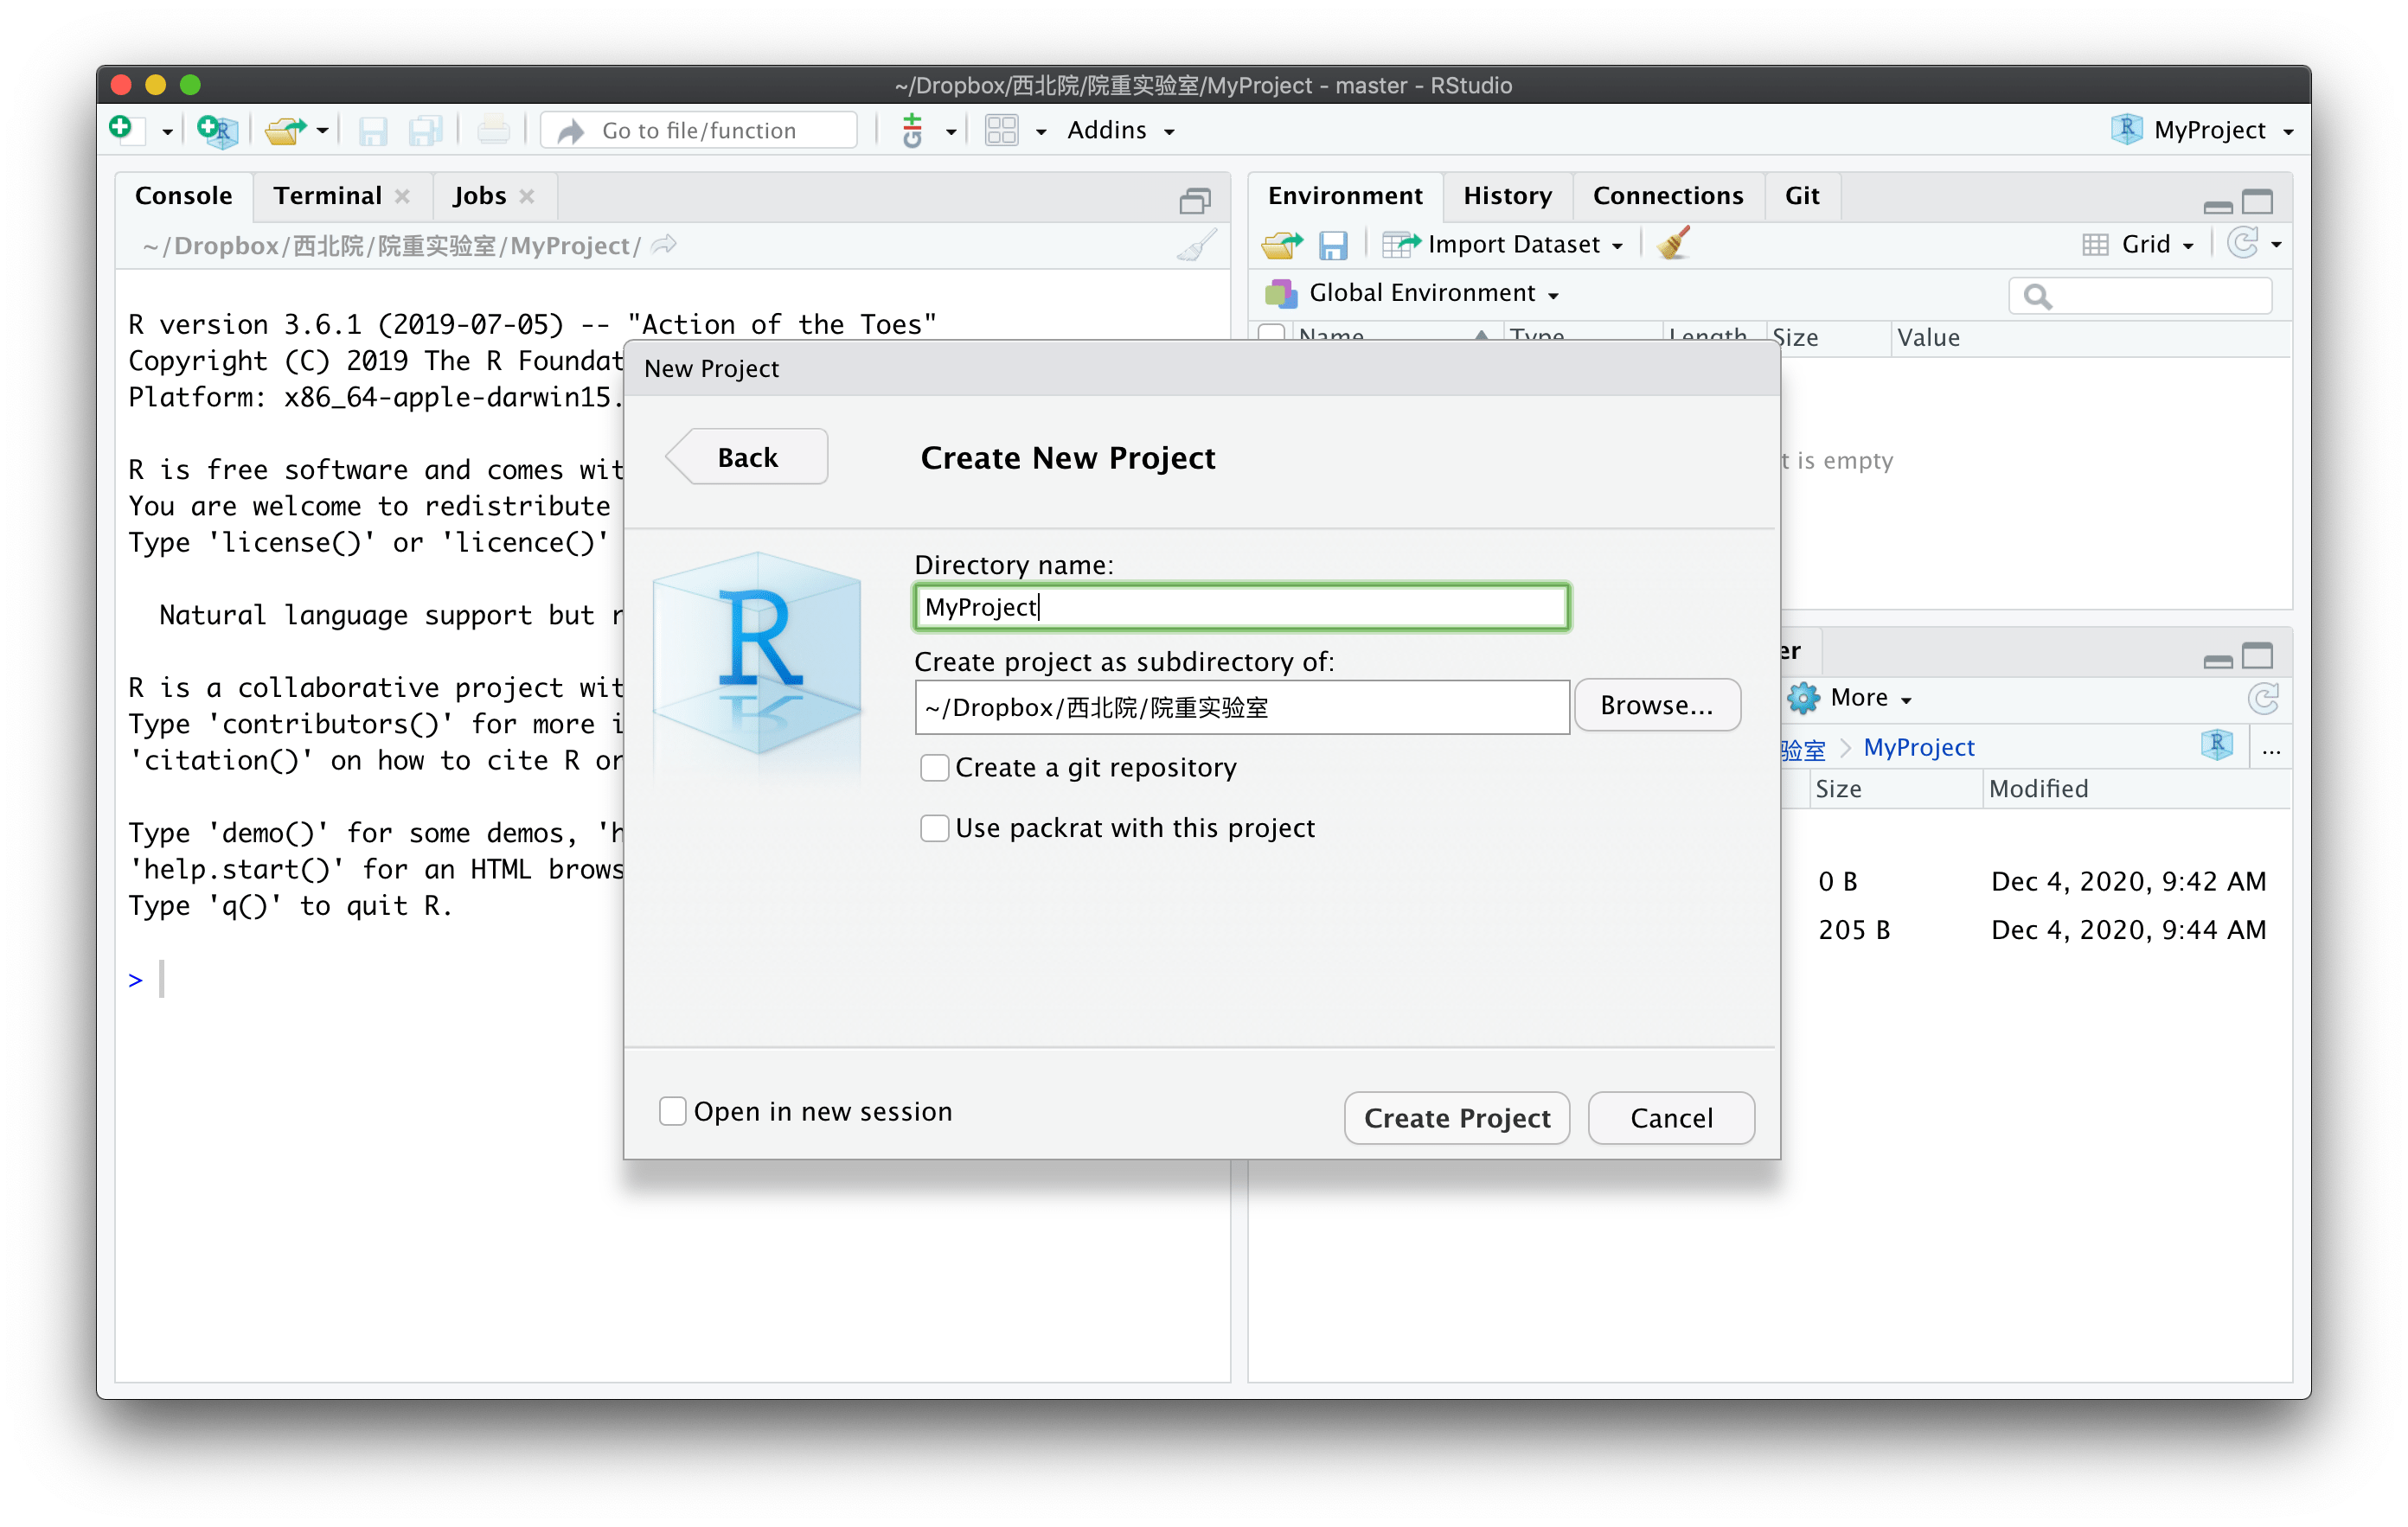
\includegraphics{Fig/ch1/Env4.png}
\caption{Env4}
\end{figure}

\begin{figure}
\centering
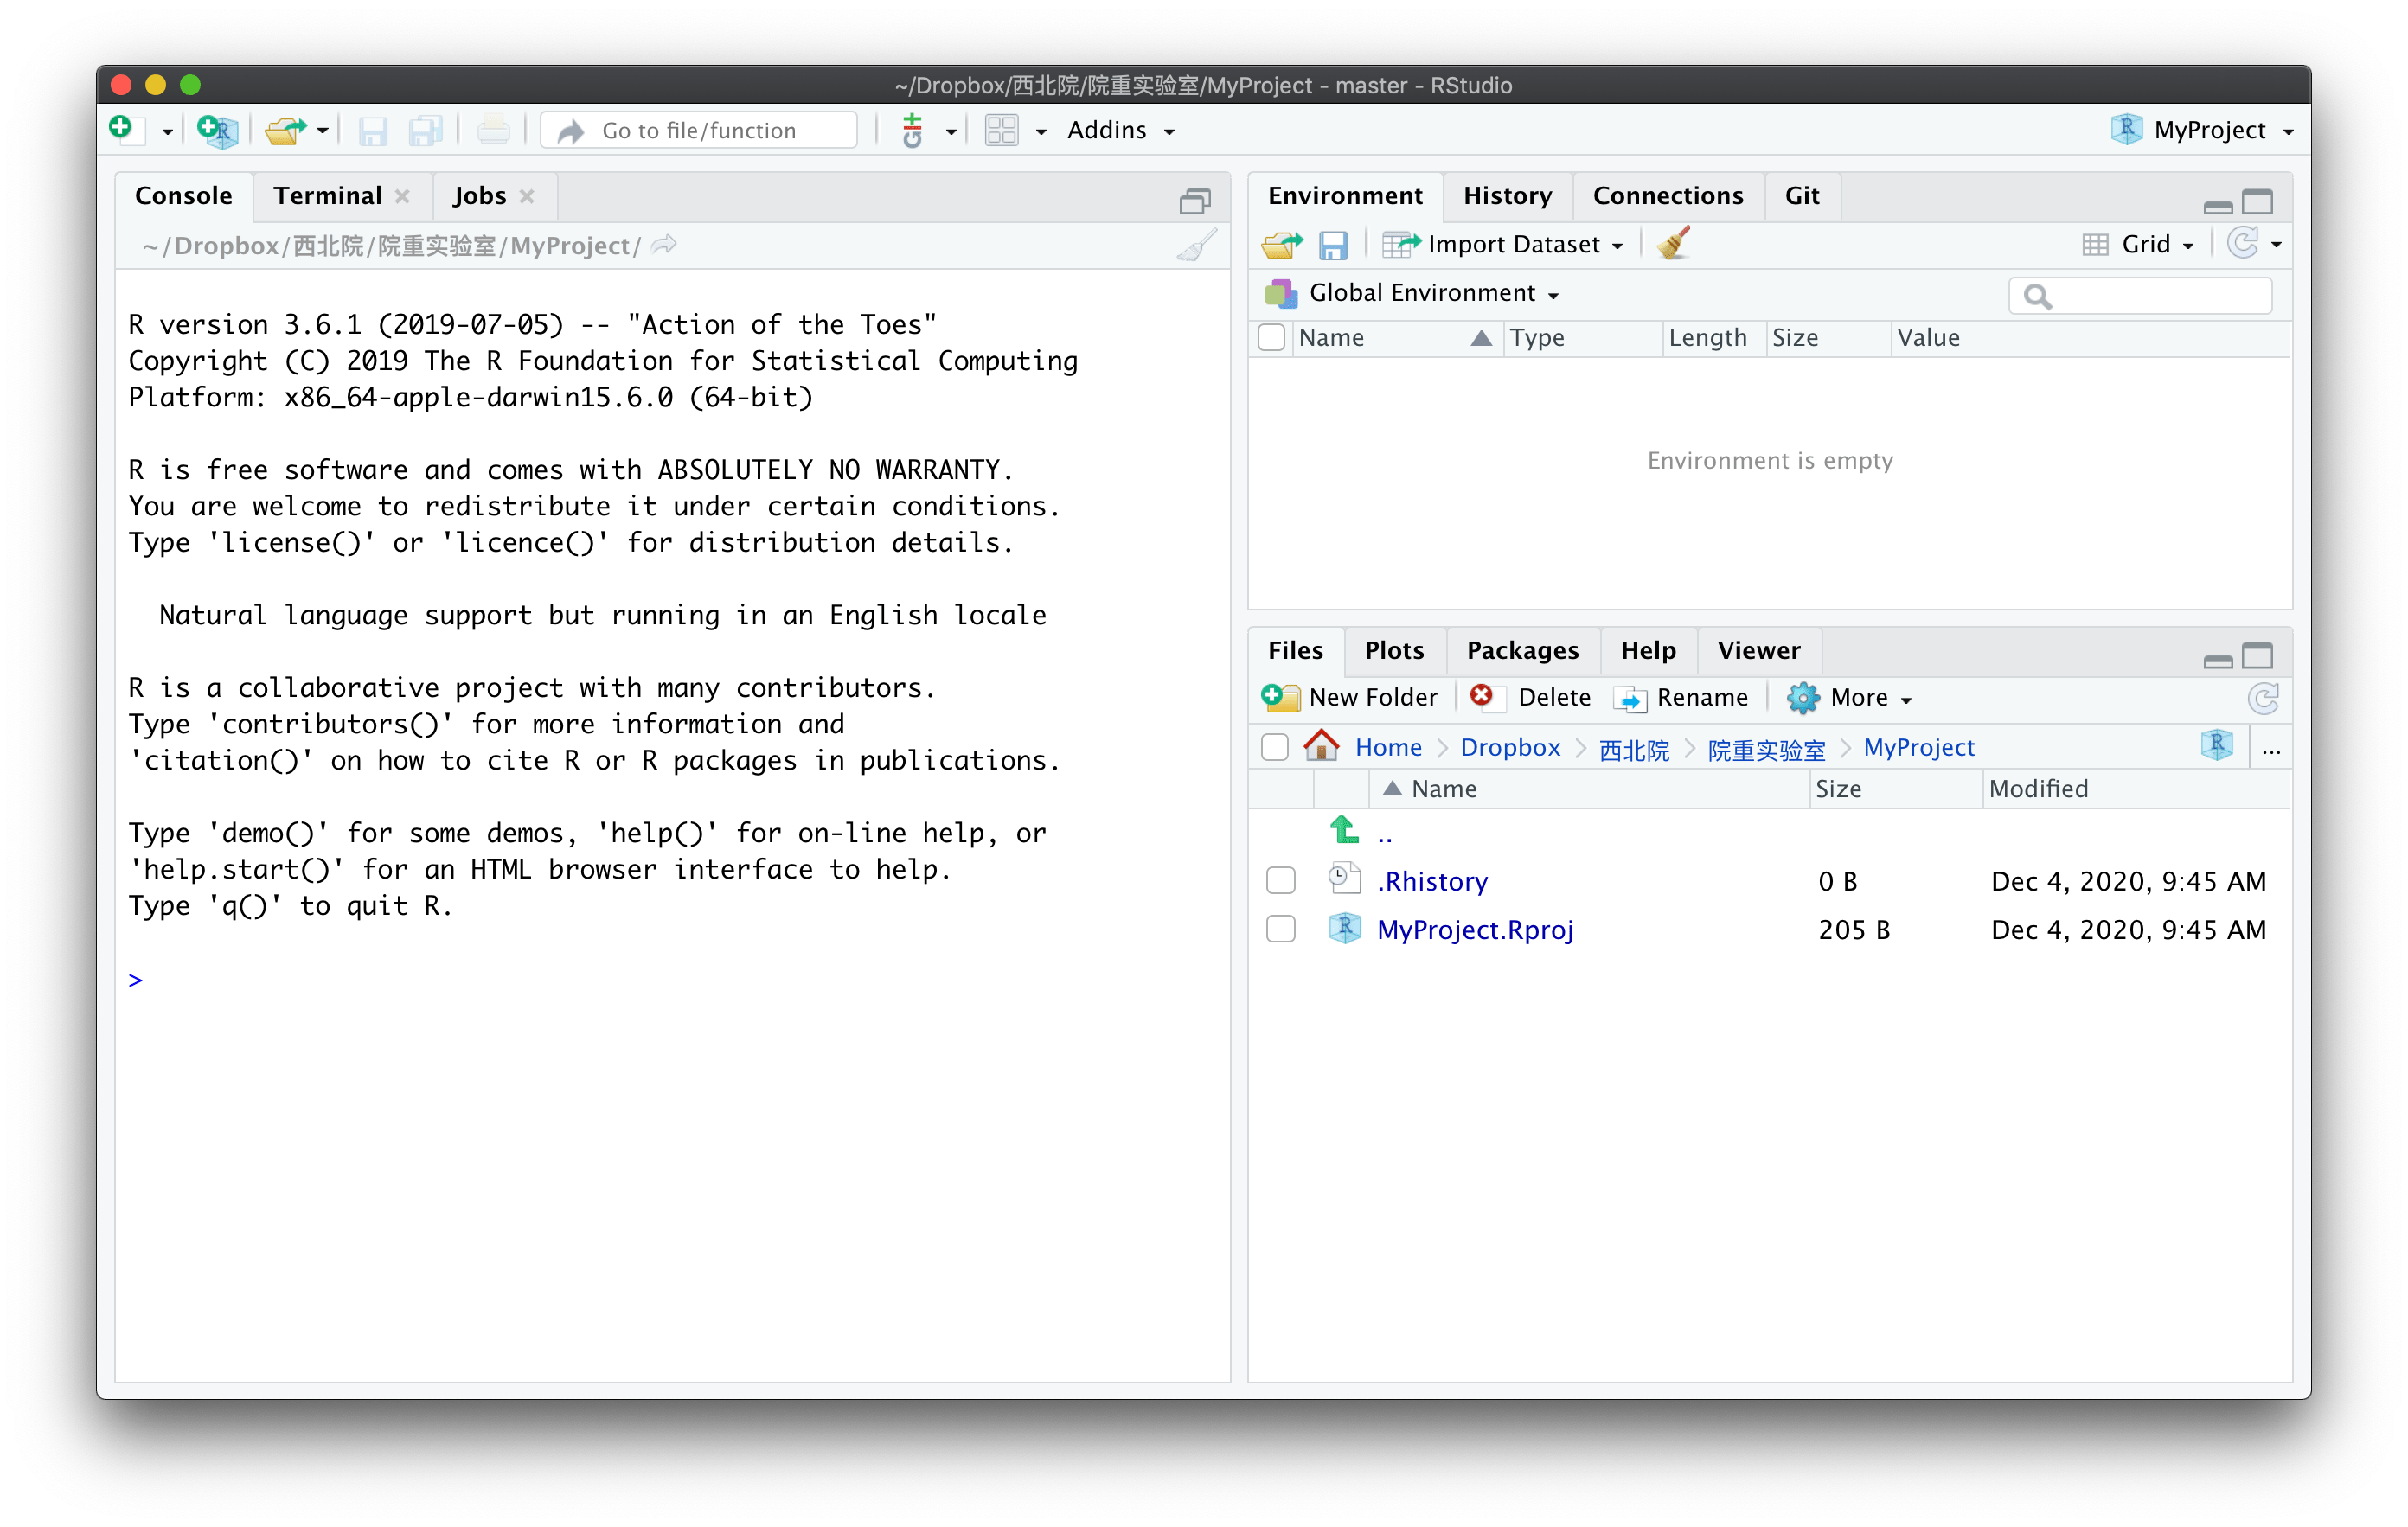
\includegraphics{Fig/ch1/Env5.png}
\caption{Env5}
\end{figure}

\begin{figure}
\centering
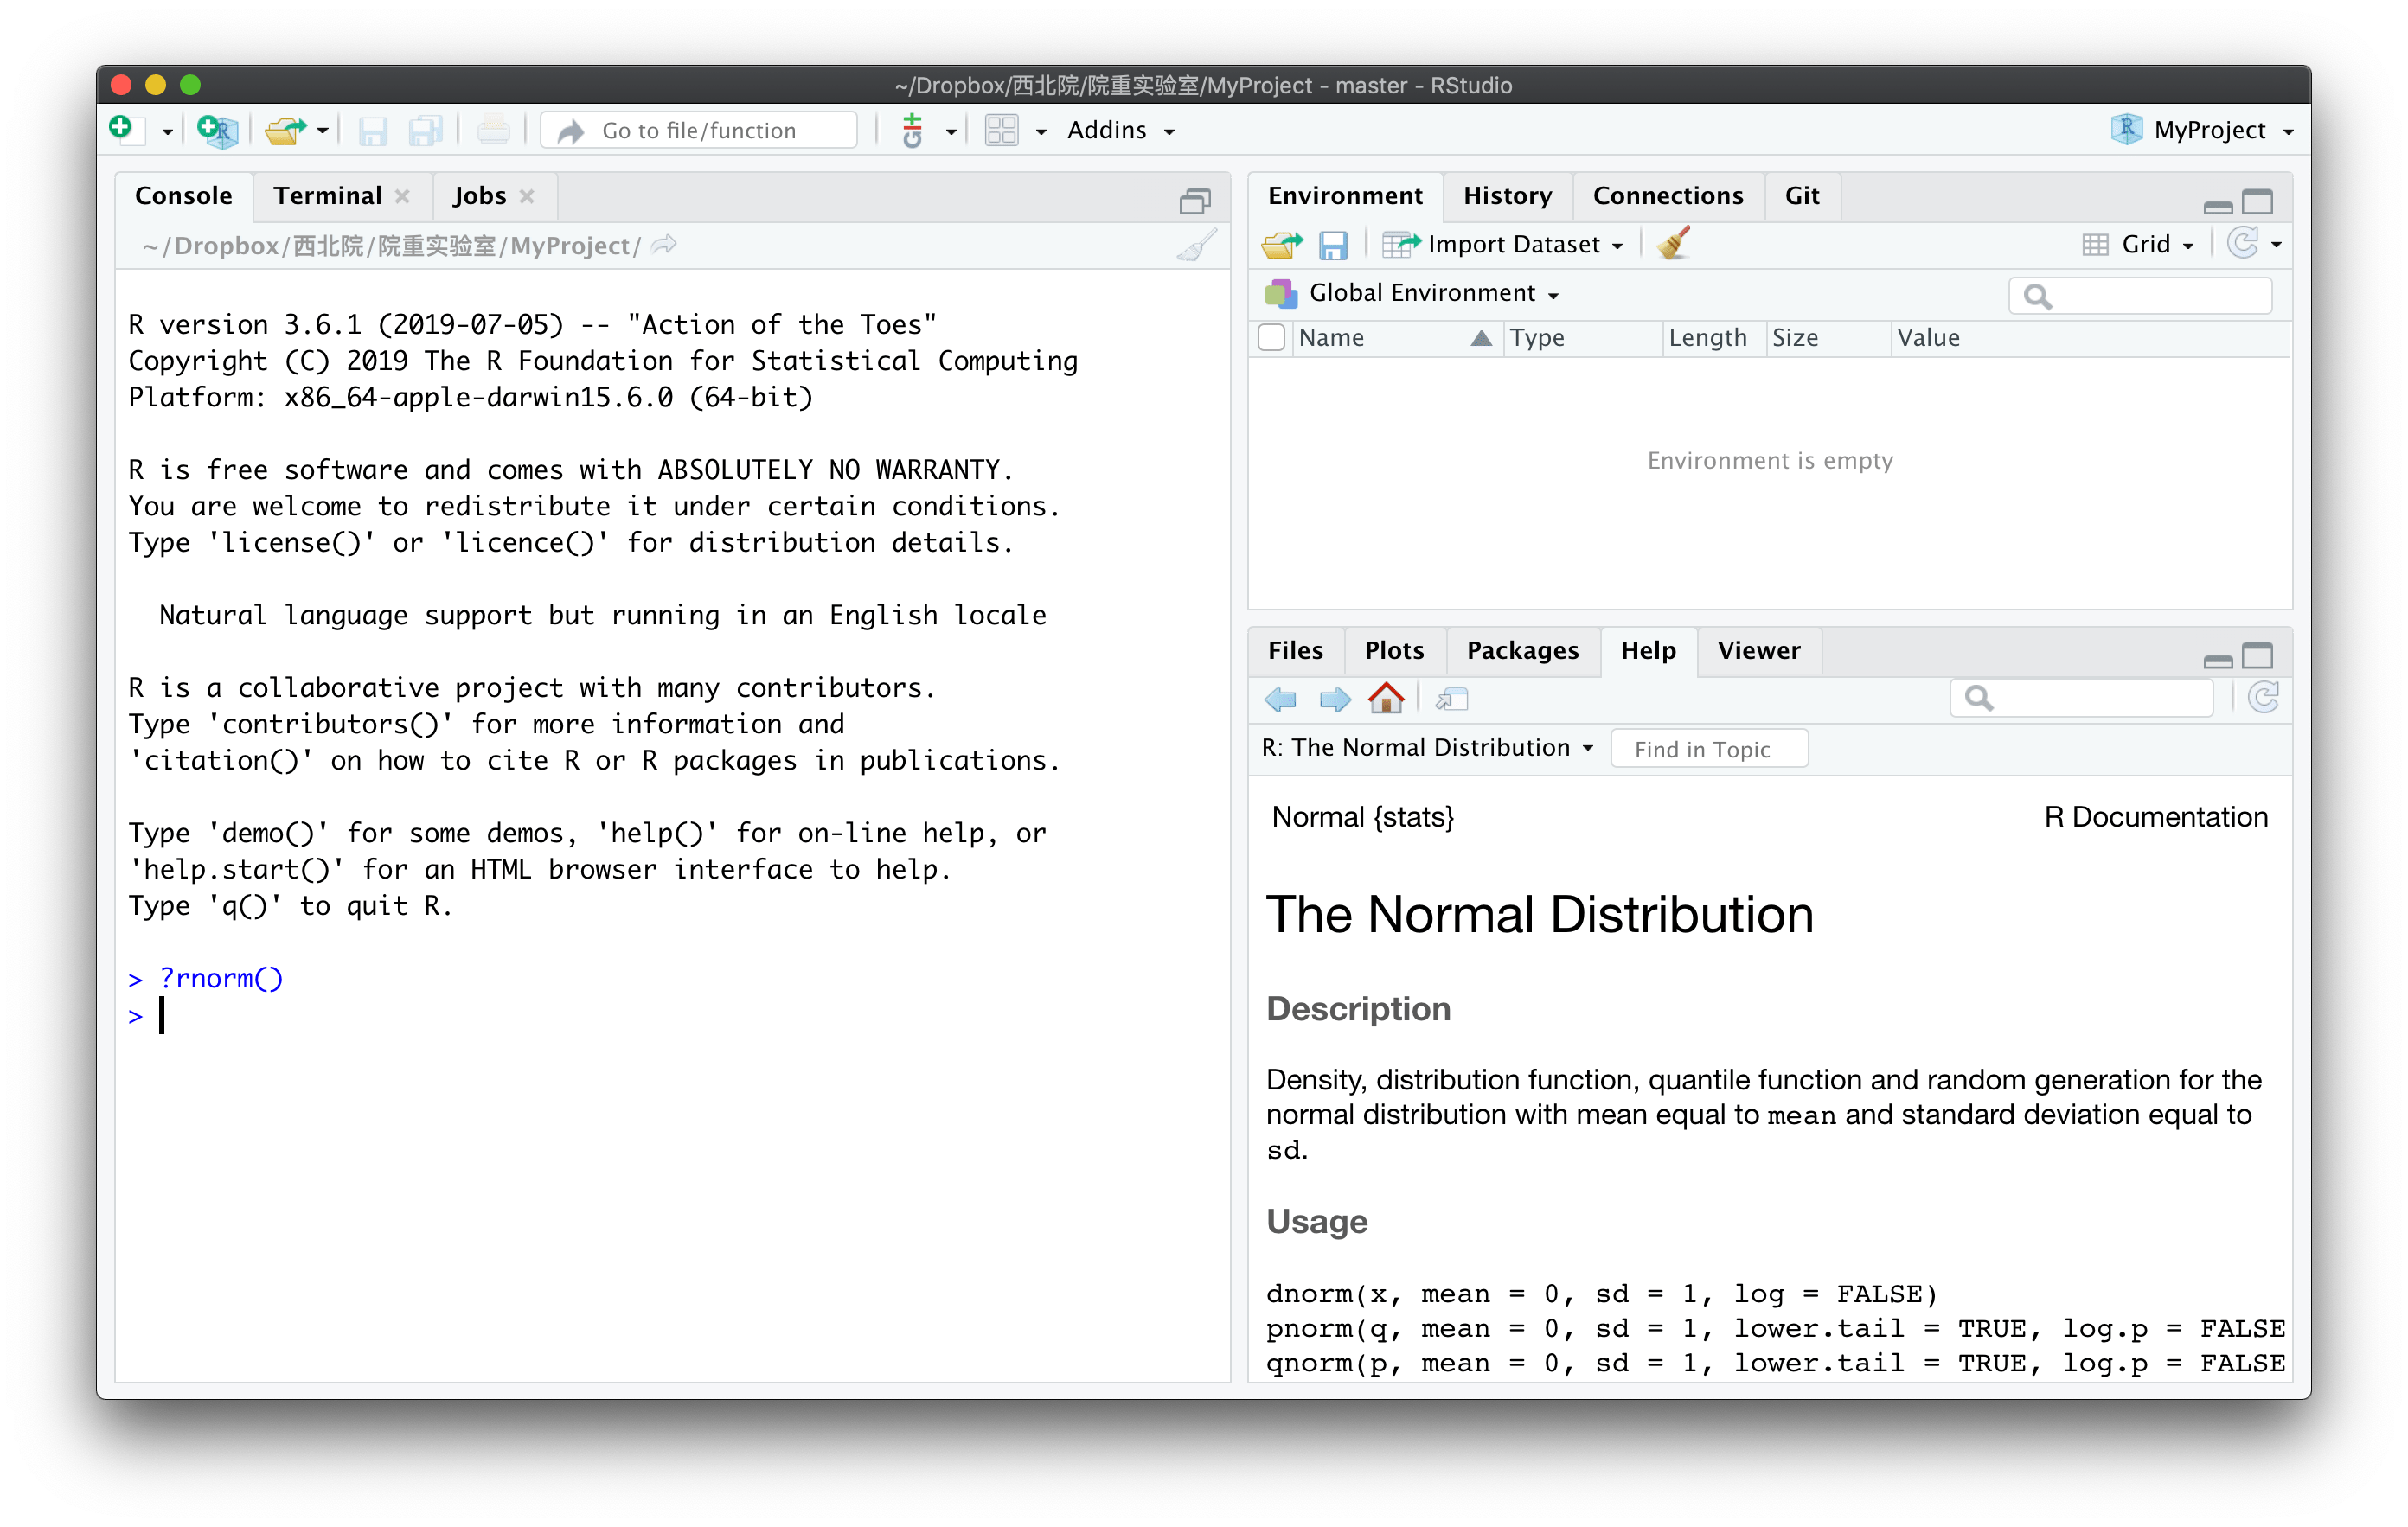
\includegraphics{Fig/ch1/Env6.png}
\caption{Env6}
\end{figure}

\begin{figure}
\centering
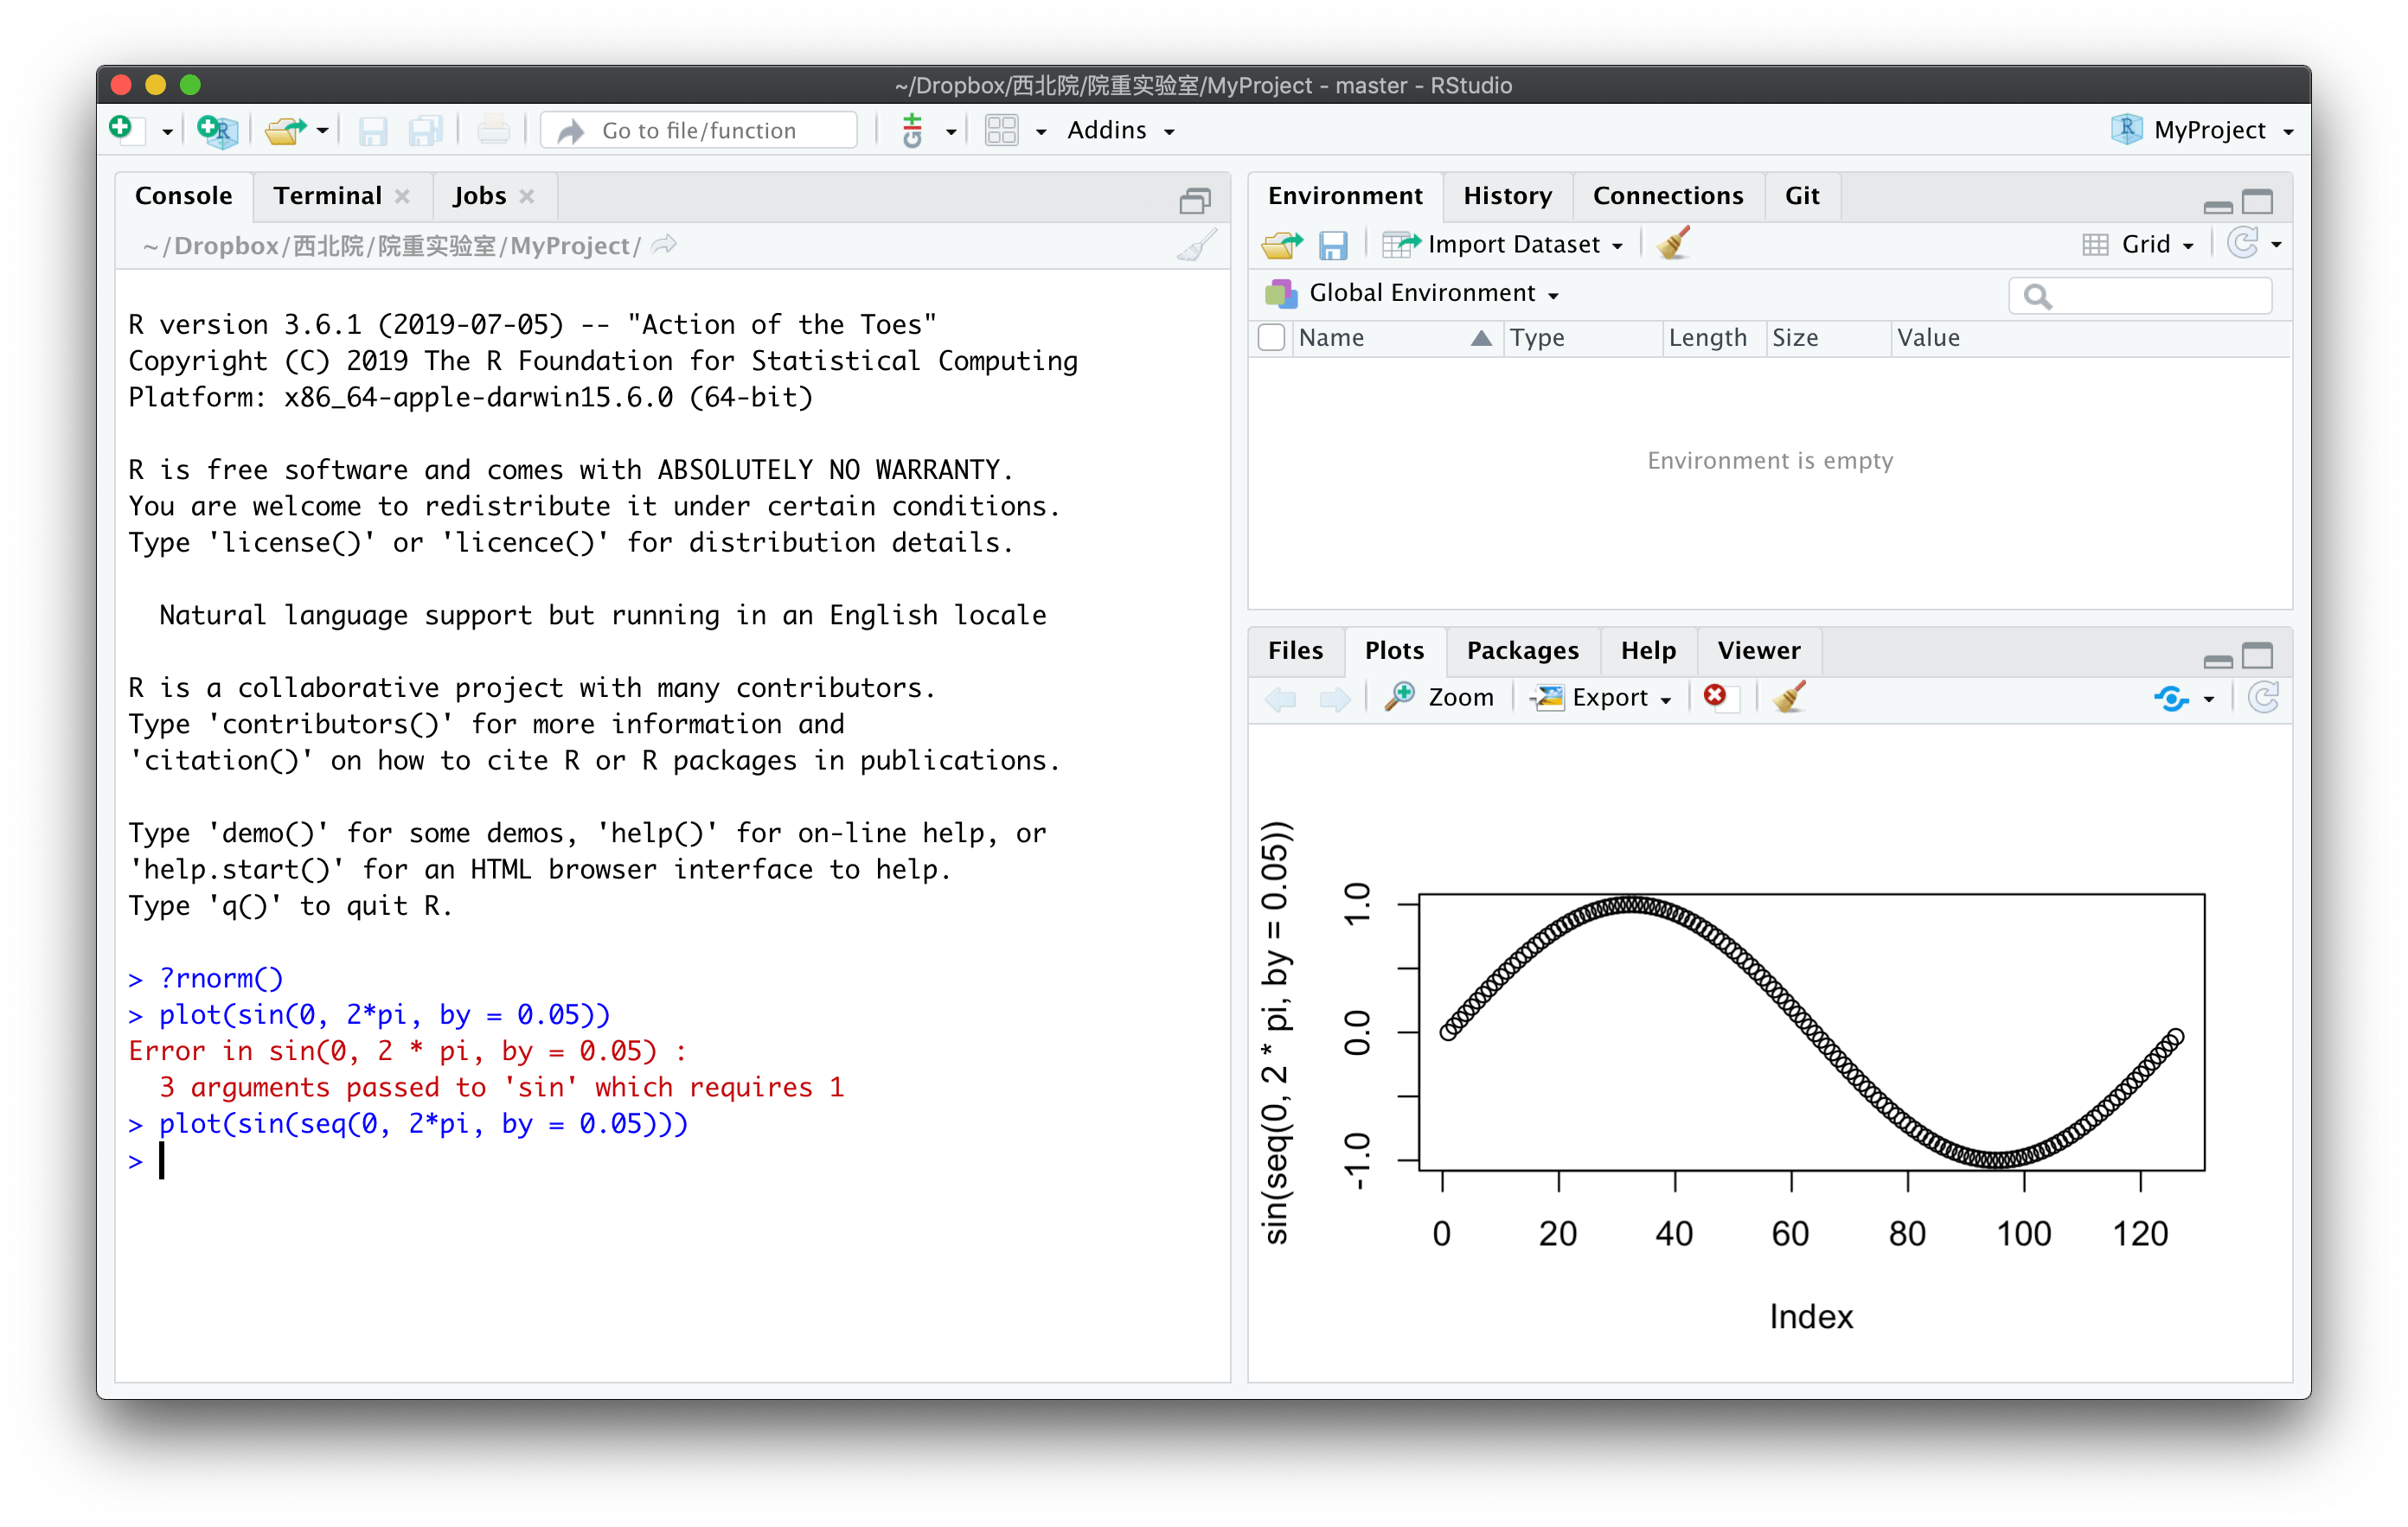
\includegraphics{Fig/ch1/Env7.png}
\caption{Env7}
\end{figure}

\hypertarget{ux5982ux4f55ux5bfbux6c42ux5e2eux52a9}{%
\section{如何寻求帮助}\label{ux5982ux4f55ux5bfbux6c42ux5e2eux52a9}}

\begin{itemize}
\item
  帮助文件
\item
  搜索
\item
  R社区
\item
  Stack Overflow
\item
  Github issure/bug
\item
  给人写信
\end{itemize}

\hypertarget{basic}{%
\chapter{R基础知识}\label{basic}}

\hypertarget{ux7f16ux7a0bux57faux7840ux8bedux6cd5}{%
\section{编程基础语法}\label{ux7f16ux7a0bux57faux7840ux8bedux6cd5}}

以下代码用于展示r的数据操作、基本数据结构和常用的函数。

\begin{Shaded}
\begin{Highlighting}[]
\NormalTok{x =}\StringTok{ }\KeywordTok{seq}\NormalTok{(}\DecValTok{1}\NormalTok{, }\DecValTok{10}\NormalTok{, }\DataTypeTok{by=}\FloatTok{0.1}\NormalTok{)  }\CommentTok{\# 生产一组数列,间隔为0.1}
\NormalTok{y =}\StringTok{ }\DecValTok{2} \OperatorTok{*}\StringTok{ }\KeywordTok{sin}\NormalTok{( x )      }\CommentTok{\# 包含 Sin 函数}
\KeywordTok{plot}\NormalTok{(x, y)      }\CommentTok{\# 绘制出(x,y)的曲线。}
\end{Highlighting}
\end{Shaded}

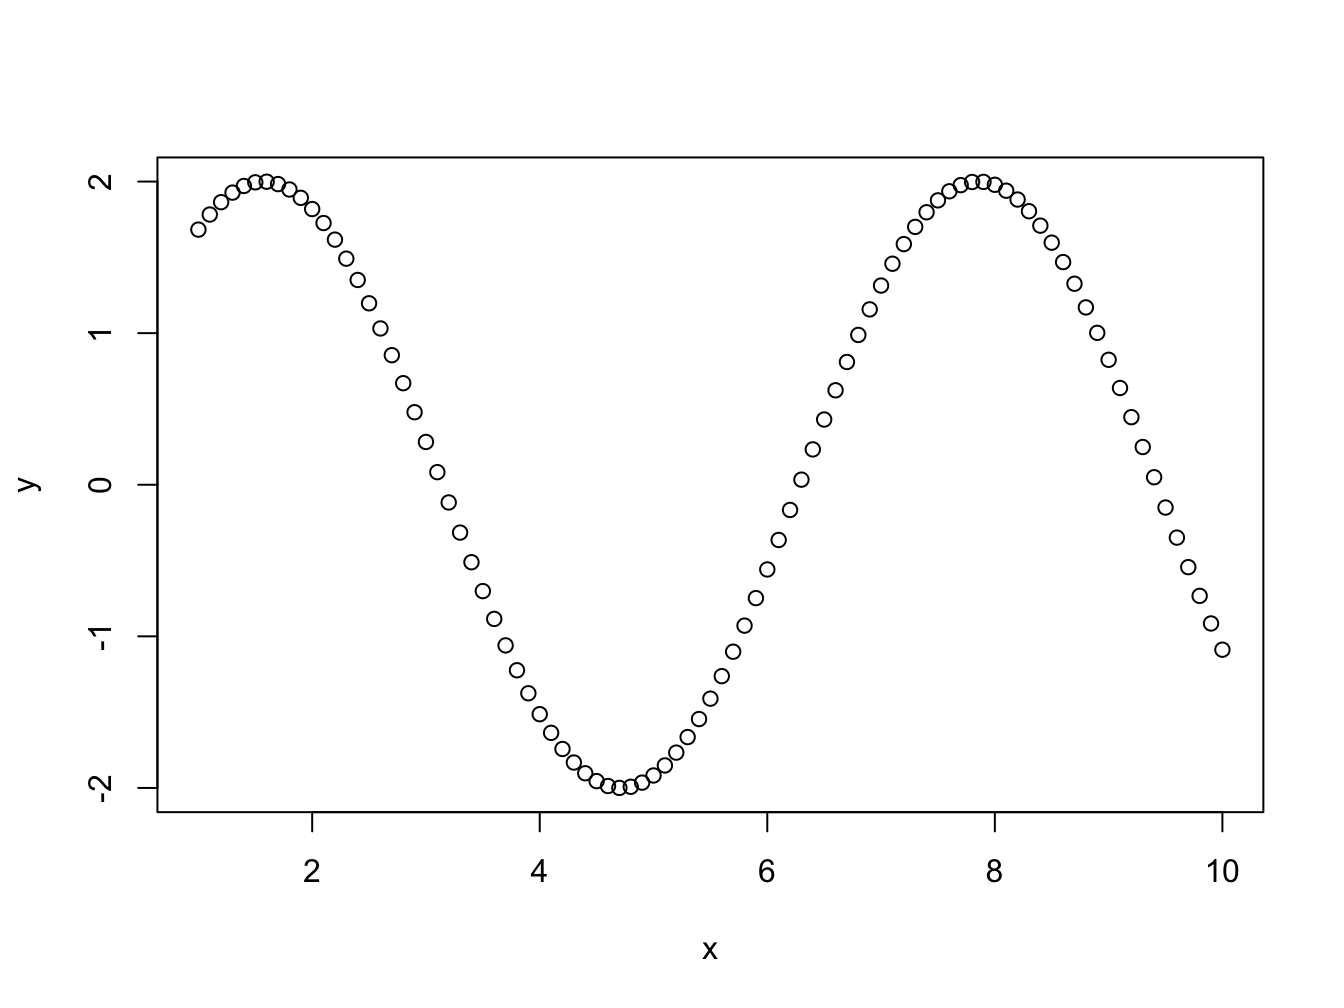
\includegraphics{R_in_Geoscience_files/figure-latex/unnamed-chunk-1-1.pdf}

\begin{Shaded}
\begin{Highlighting}[]
\KeywordTok{plot}\NormalTok{(}\DataTypeTok{x=}\NormalTok{x, }\DataTypeTok{y=}\NormalTok{y, }
     \DataTypeTok{xlab=}\StringTok{\textquotesingle{}x value\textquotesingle{}}\NormalTok{, }\DataTypeTok{ylab =} \KeywordTok{bquote}\NormalTok{(}\DecValTok{2} \OperatorTok{*}\StringTok{ }\KeywordTok{sin}\NormalTok{( x ) ), }\DataTypeTok{col=}\DecValTok{2}\NormalTok{,}
     \DataTypeTok{type=}\StringTok{\textquotesingle{}o\textquotesingle{}}\NormalTok{)}
\KeywordTok{lines}\NormalTok{(}\DataTypeTok{x=}\NormalTok{x, }\DataTypeTok{y=}\KeywordTok{abs}\NormalTok{(y), }\DataTypeTok{col=}\StringTok{\textquotesingle{}blue\textquotesingle{}}\NormalTok{)}
\KeywordTok{mtext}\NormalTok{(}\DataTypeTok{side =} \DecValTok{3}\NormalTok{, }\DataTypeTok{text =} \StringTok{\textquotesingle{}Sin(x)\textquotesingle{}}\NormalTok{, }\DataTypeTok{cex=}\DecValTok{2}\NormalTok{, }\DataTypeTok{line=}\OperatorTok{{-}}\DecValTok{2}\NormalTok{)}
\KeywordTok{grid}\NormalTok{()}
\end{Highlighting}
\end{Shaded}

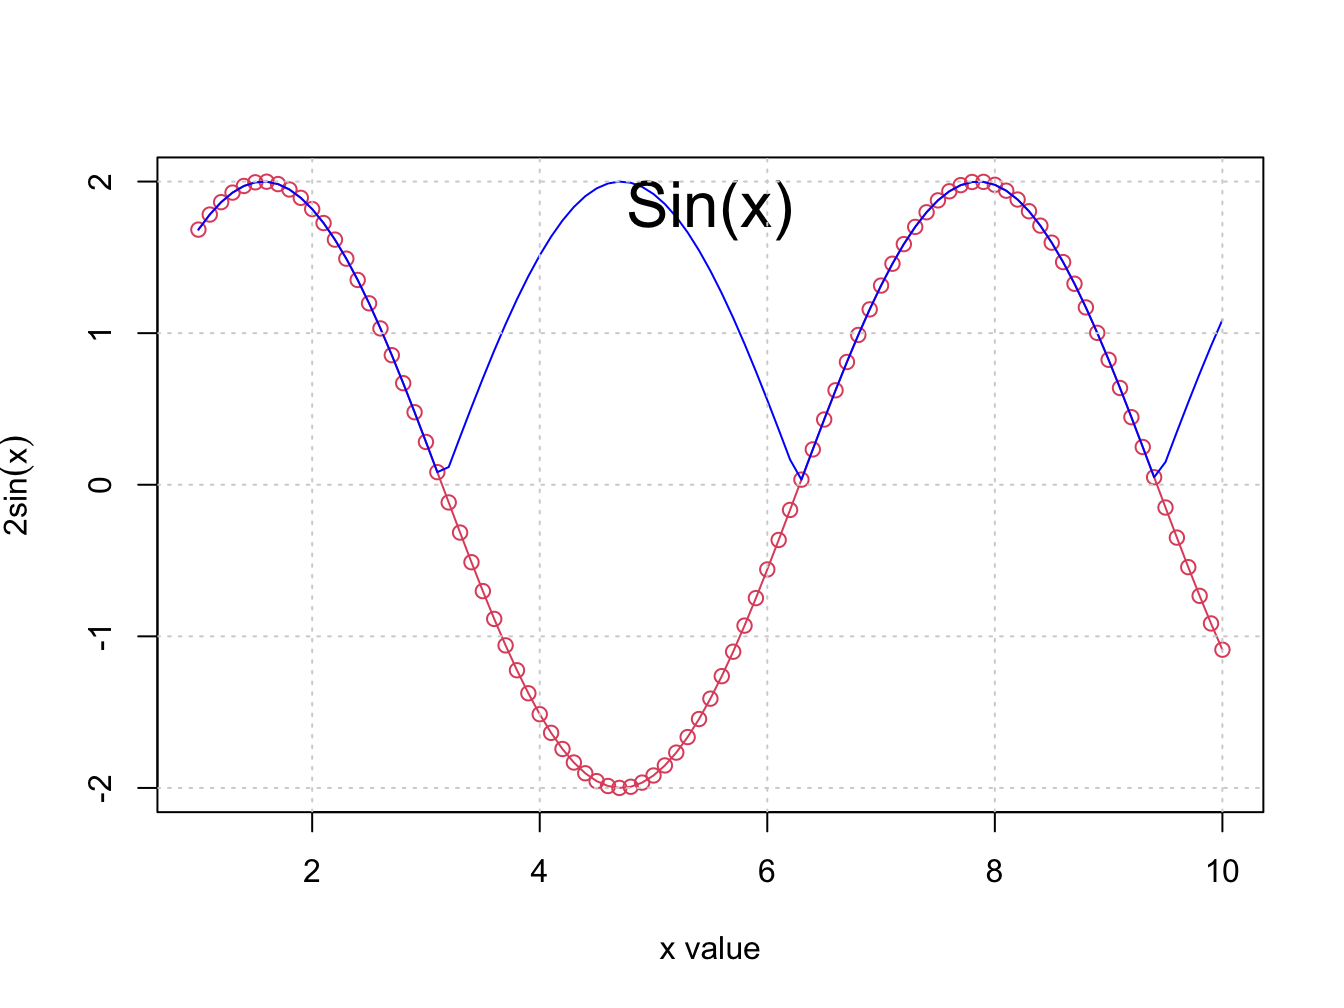
\includegraphics{R_in_Geoscience_files/figure-latex/unnamed-chunk-1-2.pdf}

\begin{Shaded}
\begin{Highlighting}[]
\KeywordTok{length}\NormalTok{(x)}
\end{Highlighting}
\end{Shaded}

\begin{verbatim}
## [1] 91
\end{verbatim}

\begin{Shaded}
\begin{Highlighting}[]
\NormalTok{mat.v =}\StringTok{ }\KeywordTok{cbind}\NormalTok{(x, y)}
\NormalTok{mat.h =}\StringTok{ }\KeywordTok{rbind}\NormalTok{(x, y)}

\KeywordTok{boxplot}\NormalTok{(mat.v)}
\end{Highlighting}
\end{Shaded}

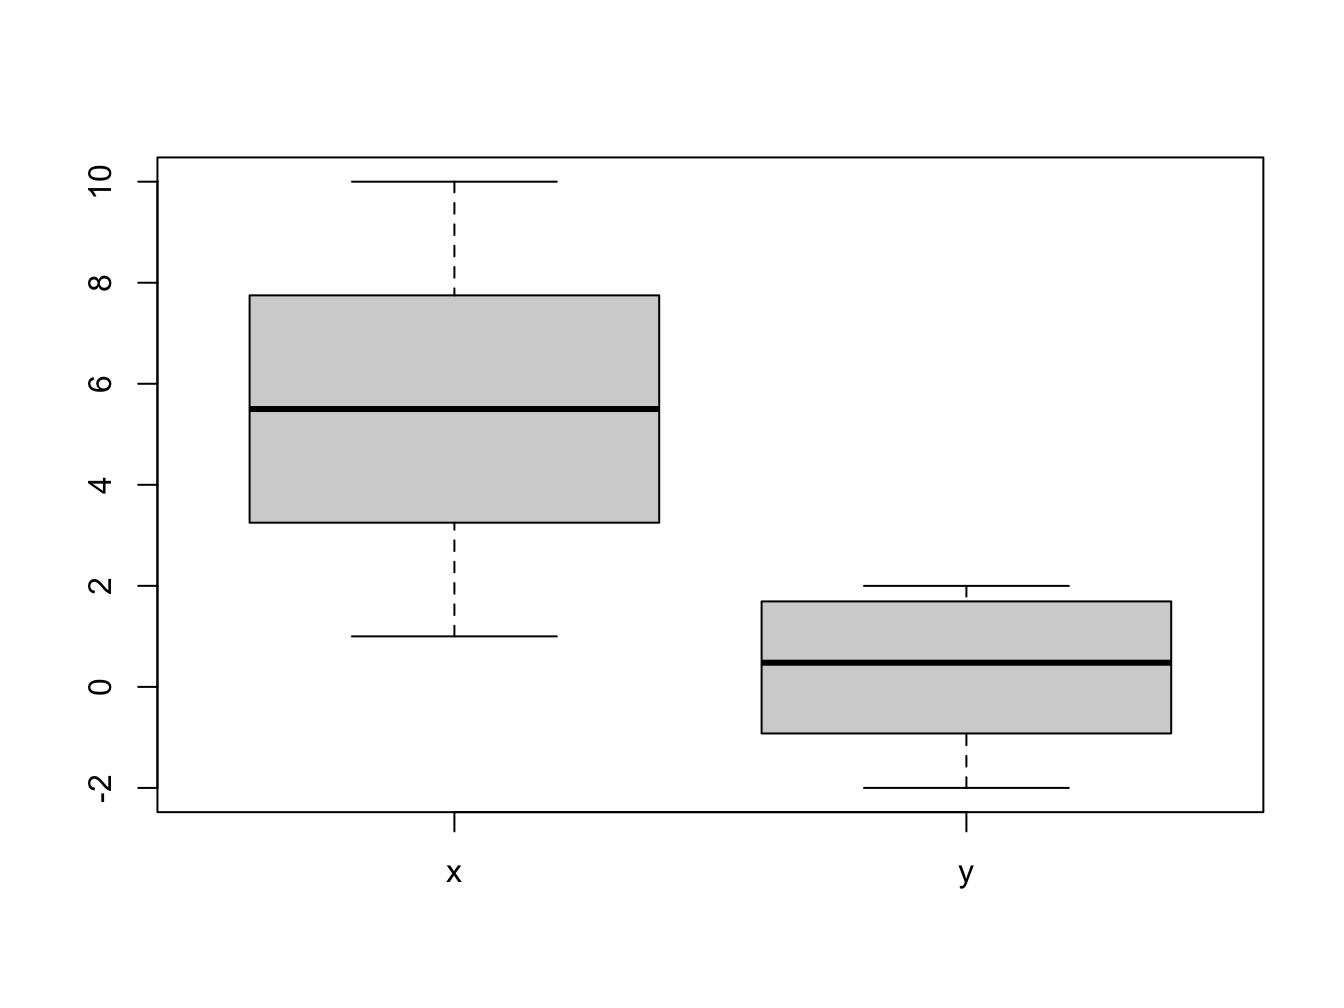
\includegraphics{R_in_Geoscience_files/figure-latex/unnamed-chunk-1-3.pdf}

\begin{Shaded}
\begin{Highlighting}[]
\KeywordTok{class}\NormalTok{(mat.v)}
\end{Highlighting}
\end{Shaded}

\begin{verbatim}
## [1] "matrix"
\end{verbatim}

\begin{Shaded}
\begin{Highlighting}[]
\KeywordTok{dim}\NormalTok{(mat.v)}
\end{Highlighting}
\end{Shaded}

\begin{verbatim}
## [1] 91  2
\end{verbatim}

\begin{Shaded}
\begin{Highlighting}[]
\KeywordTok{dim}\NormalTok{(mat.h)}
\end{Highlighting}
\end{Shaded}

\begin{verbatim}
## [1]  2 91
\end{verbatim}

\begin{Shaded}
\begin{Highlighting}[]
\KeywordTok{nrow}\NormalTok{(mat.v)}
\end{Highlighting}
\end{Shaded}

\begin{verbatim}
## [1] 91
\end{verbatim}

\begin{Shaded}
\begin{Highlighting}[]
\KeywordTok{ncol}\NormalTok{(mat.v)}
\end{Highlighting}
\end{Shaded}

\begin{verbatim}
## [1] 2
\end{verbatim}

\hypertarget{ux51fdux6570ux5b9aux4e49}{%
\subsection{函数定义}\label{ux51fdux6570ux5b9aux4e49}}

文件1\texttt{Excercise/Functions/fun.add.R}内容:

\begin{Shaded}
\begin{Highlighting}[]
\NormalTok{fun.add \textless{}{-}}\StringTok{ }\ControlFlowTok{function}\NormalTok{(a, b)\{}
  \KeywordTok{return}\NormalTok{ (a }\OperatorTok{+}\StringTok{ }\NormalTok{b)}
\NormalTok{\}}
\end{Highlighting}
\end{Shaded}

文件2\texttt{add.R}内容:

\begin{Shaded}
\begin{Highlighting}[]
\KeywordTok{source}\NormalTok{(}\StringTok{\textquotesingle{}Excercise/Functions/fun.add.R\textquotesingle{}}\NormalTok{)}
\KeywordTok{fun.add}\NormalTok{(}\DecValTok{2}\NormalTok{, }\DecValTok{3}\NormalTok{)}
\end{Highlighting}
\end{Shaded}

\begin{verbatim}
## [1] 5
\end{verbatim}

\hypertarget{ux6587ux4ef6ux7ba1ux7406}{%
\subsection{文件管理}\label{ux6587ux4ef6ux7ba1ux7406}}

\hypertarget{ux6570ux636eux7c7bux578bux4e0eux7ed3ux6784}{%
\section{数据类型与结构}\label{ux6570ux636eux7c7bux578bux4e0eux7ed3ux6784}}

\begin{enumerate}
\def\labelenumi{\arabic{enumi}.}
\tightlist
\item
  数字:numeric
  即一维数组, 常用的函数\texttt{length}, \texttt{class}等。
\end{enumerate}

\begin{Shaded}
\begin{Highlighting}[]
\NormalTok{x0 =}\StringTok{ }\KeywordTok{rnorm}\NormalTok{(}\DecValTok{100}\NormalTok{)}
\KeywordTok{plot}\NormalTok{(x0)}
\end{Highlighting}
\end{Shaded}

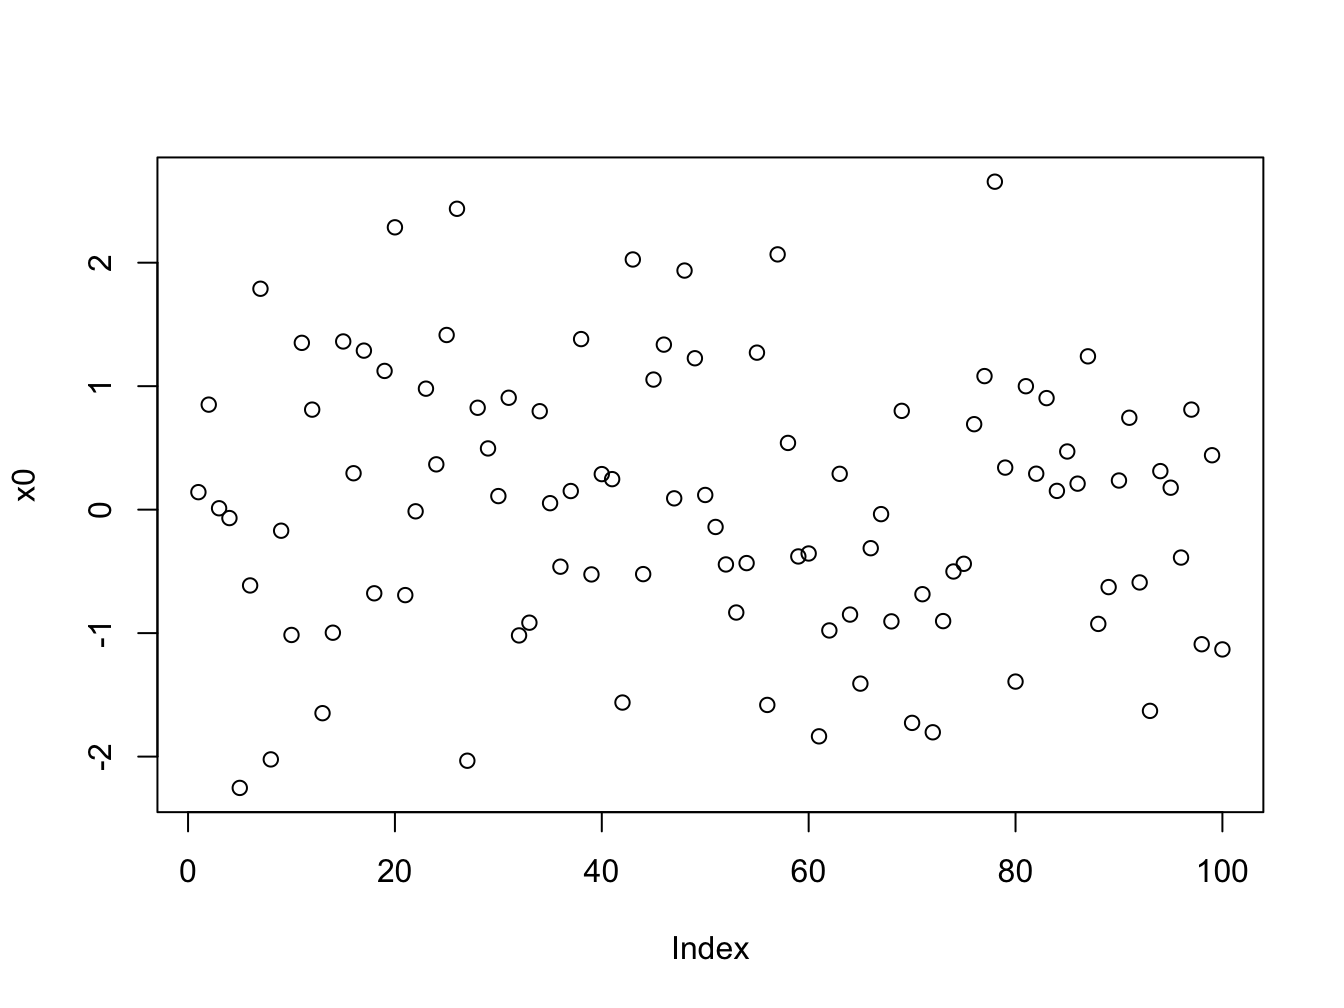
\includegraphics{R_in_Geoscience_files/figure-latex/unnamed-chunk-5-1.pdf}

\begin{enumerate}
\def\labelenumi{\arabic{enumi}.}
\tightlist
\item
  数据框:data.frame
\end{enumerate}

\begin{Shaded}
\begin{Highlighting}[]
\NormalTok{x=}\KeywordTok{readRDS}\NormalTok{(}\StringTok{\textquotesingle{}Excercise/Data\_RDS/JCR.RDS\textquotesingle{}}\NormalTok{)}
\KeywordTok{length}\NormalTok{(x)}
\end{Highlighting}
\end{Shaded}

\begin{verbatim}
## [1] 6
\end{verbatim}

\begin{Shaded}
\begin{Highlighting}[]
\KeywordTok{dim}\NormalTok{(x)}
\end{Highlighting}
\end{Shaded}

\begin{verbatim}
## [1] 14492     6
\end{verbatim}

\begin{Shaded}
\begin{Highlighting}[]
\KeywordTok{head}\NormalTok{(x) }\CommentTok{\#前5组元素}
\end{Highlighting}
\end{Shaded}

\begin{verbatim}
##          c1
## 1 Acoustics
## 2 Acoustics
## 3 Acoustics
## 4 Acoustics
## 5 Acoustics
## 6 Acoustics
##                                                                    name
## 1                                             Ultrasonics Sonochemistry
## 2                                 Ultrasound In Obstetrics & Gynecology
## 3                                            Ultraschall In Der Medizin
## 4         Ieee-acm Transactions On Audio Speech And Language Processing
## 5                                        Journal Of Sound And Vibration
## 6 Ieee Transactions On Ultrasonics Ferroelectrics And Frequency Control
##        ISSN cites    IF CR
## 1 1350-4177 17314 7.279  1
## 2 0960-7692 12336 5.595  1
## 3 0172-4614  2238 4.613  3
## 4 2329-9290  3110 3.531  2
## 5 0022-460X 36167 3.123  1
## 6 0885-3010 11266 2.989  1
\end{verbatim}

\begin{Shaded}
\begin{Highlighting}[]
\KeywordTok{View}\NormalTok{(x)}
\end{Highlighting}
\end{Shaded}

\begin{enumerate}
\def\labelenumi{\arabic{enumi}.}
\tightlist
\item
  字符:character
\end{enumerate}

\begin{Shaded}
\begin{Highlighting}[]
\KeywordTok{levels}\NormalTok{(x}\OperatorTok{$}\NormalTok{name)[}\DecValTok{1}\OperatorTok{:}\DecValTok{5}\NormalTok{]}
\end{Highlighting}
\end{Shaded}

\begin{verbatim}
## [1] ""                                              
## [2] "2d Materials"                                  
## [3] "3 Biotech"                                     
## [4] "3d Printing And Additive Manufacturing"        
## [5] "4or-a Quarterly Journal Of Operations Research"
\end{verbatim}

\begin{enumerate}
\def\labelenumi{\arabic{enumi}.}
\tightlist
\item
  向量:vector
\end{enumerate}

\begin{Shaded}
\begin{Highlighting}[]
\NormalTok{vec =}\StringTok{ }\KeywordTok{cbind}\NormalTok{(}\DecValTok{1}\OperatorTok{:}\DecValTok{10}\NormalTok{)}
\KeywordTok{plot}\NormalTok{(vec)}
\end{Highlighting}
\end{Shaded}

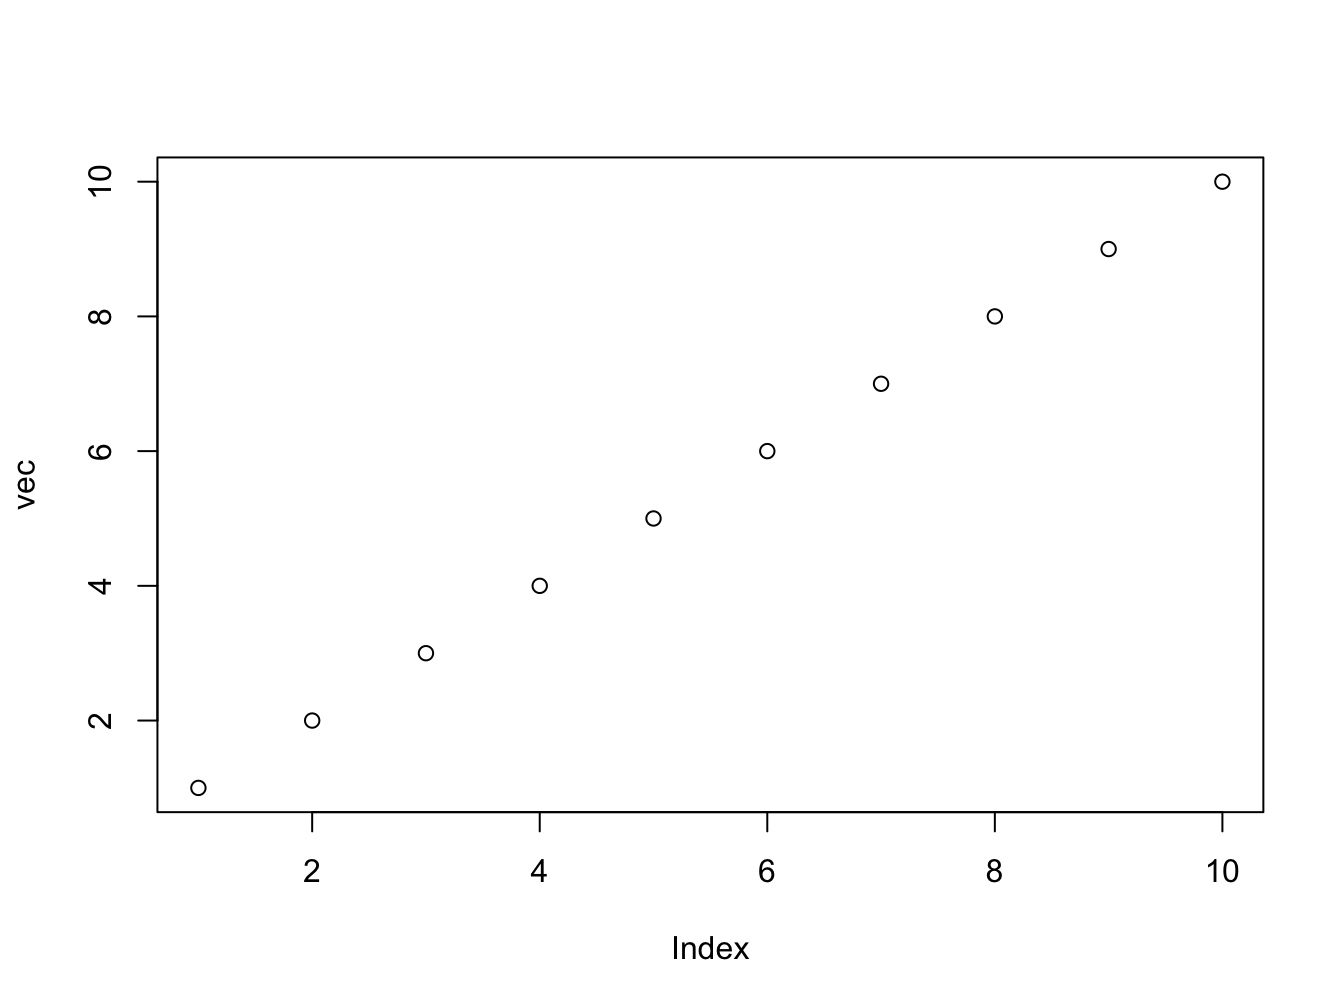
\includegraphics{R_in_Geoscience_files/figure-latex/unnamed-chunk-9-1.pdf}
1. 矩阵:matrix

\begin{Shaded}
\begin{Highlighting}[]
\NormalTok{x.mat =}\StringTok{ }\KeywordTok{as.matrix}\NormalTok{(x)}
\KeywordTok{class}\NormalTok{(x.mat)}
\end{Highlighting}
\end{Shaded}

\begin{verbatim}
## [1] "matrix"
\end{verbatim}

\begin{Shaded}
\begin{Highlighting}[]
\KeywordTok{length}\NormalTok{(x.mat)}
\end{Highlighting}
\end{Shaded}

\begin{verbatim}
## [1] 86952
\end{verbatim}

\begin{enumerate}
\def\labelenumi{\arabic{enumi}.}
\tightlist
\item
  因子:factor
\end{enumerate}

\begin{Shaded}
\begin{Highlighting}[]
\KeywordTok{library}\NormalTok{(ggplot2)}
\KeywordTok{head}\NormalTok{(}\KeywordTok{levels}\NormalTok{(x}\OperatorTok{$}\NormalTok{c1))}
\end{Highlighting}
\end{Shaded}

\begin{verbatim}
## [1] "Acoustics"                          
## [2] "Agricultural Economics & Policy"    
## [3] "Agricultural Engineering"           
## [4] "Agriculture, Dairy & Animal Science"
## [5] "Agriculture, Multidisciplinary"     
## [6] "Agronomy"
\end{verbatim}

\begin{enumerate}
\def\labelenumi{\arabic{enumi}.}
\tightlist
\item
  逻辑:logical
\end{enumerate}

\begin{Shaded}
\begin{Highlighting}[]
\NormalTok{x =}\StringTok{ }\KeywordTok{seq}\NormalTok{(}\OperatorTok{{-}}\NormalTok{pi}\OperatorTok{*}\DecValTok{2}\NormalTok{, pi }\OperatorTok{*}\StringTok{ }\DecValTok{2}\NormalTok{, }\DataTypeTok{by=}\FloatTok{0.01}\NormalTok{)}
\NormalTok{y =}\StringTok{ }\KeywordTok{sin}\NormalTok{(x)}
\NormalTok{tf =}\StringTok{ }\NormalTok{(y }\OperatorTok{\textgreater{}}\StringTok{ }\DecValTok{0}\NormalTok{)}
\NormalTok{df =}\StringTok{ }\KeywordTok{data.frame}\NormalTok{(x, y, tf)}

\KeywordTok{plot}\NormalTok{(x, y, }\DataTypeTok{type =} \StringTok{\textquotesingle{}o\textquotesingle{}}\NormalTok{, }\DataTypeTok{pch =} \DecValTok{19}\NormalTok{, }\DataTypeTok{col =}\NormalTok{ tf}\OperatorTok{+}\DecValTok{1}\NormalTok{, }\DataTypeTok{xlab=}\StringTok{\textquotesingle{}X\textquotesingle{}}\NormalTok{, }\DataTypeTok{ylab =} \StringTok{\textquotesingle{}Y = sin(x)\textquotesingle{}}\NormalTok{)}
\KeywordTok{abline}\NormalTok{(}\DataTypeTok{v =} \DecValTok{0}\NormalTok{, }\DataTypeTok{col=}\StringTok{\textquotesingle{}red\textquotesingle{}}\NormalTok{, }\DataTypeTok{lwd=}\DecValTok{4}\NormalTok{) }\CommentTok{\#在x = 0处添加垂直线条,}
\KeywordTok{abline}\NormalTok{(}\DataTypeTok{h =} \DecValTok{0}\NormalTok{, }\DataTypeTok{col=}\StringTok{\textquotesingle{}blue\textquotesingle{}}\NormalTok{, }\DataTypeTok{lwd=}\DecValTok{4}\NormalTok{) }\CommentTok{\#在y = 0处添加水平线条,}
\KeywordTok{grid}\NormalTok{()  }\CommentTok{\# 添加坐标网格}
\end{Highlighting}
\end{Shaded}

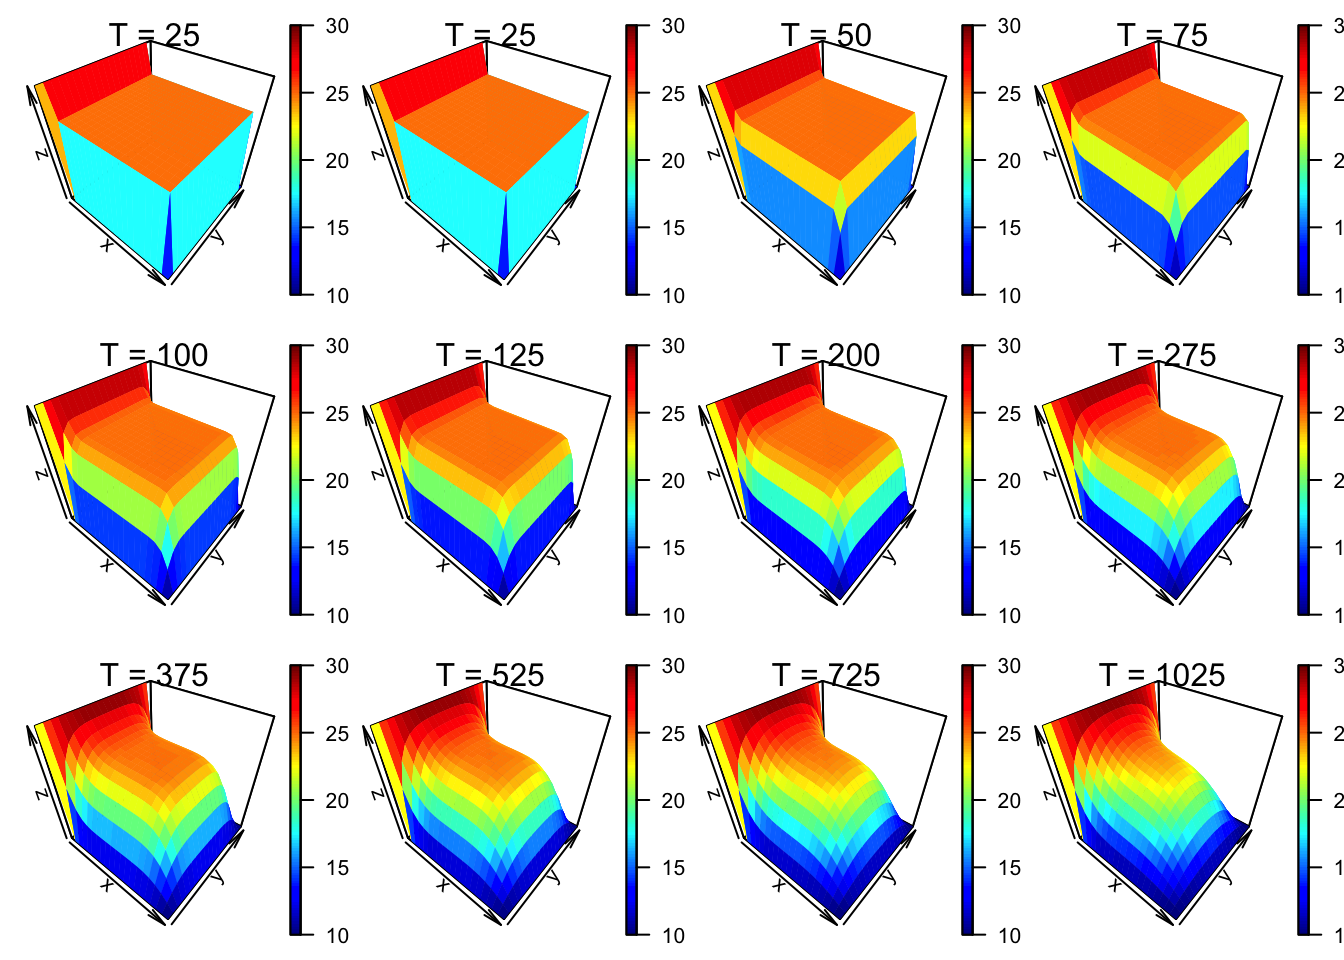
\includegraphics{R_in_Geoscience_files/figure-latex/unnamed-chunk-12-1.pdf}

\hypertarget{ux53efux89c6ux5316}{%
\section{可视化}\label{ux53efux89c6ux5316}}

\begin{Shaded}
\begin{Highlighting}[]
\KeywordTok{par}\NormalTok{(}\DataTypeTok{mar =} \KeywordTok{c}\NormalTok{(}\DecValTok{4}\NormalTok{, }\DecValTok{4}\NormalTok{, }\FloatTok{.1}\NormalTok{, }\FloatTok{.1}\NormalTok{))  }\CommentTok{\# 绘图的四边边界}
\NormalTok{x =}\StringTok{ }\KeywordTok{seq}\NormalTok{(}\OperatorTok{{-}}\NormalTok{pi}\OperatorTok{*}\DecValTok{2}\NormalTok{, pi }\OperatorTok{*}\StringTok{ }\DecValTok{2}\NormalTok{, }\DataTypeTok{by=}\FloatTok{0.01}\NormalTok{)}
\NormalTok{y =}\StringTok{ }\KeywordTok{sin}\NormalTok{(x)}
\KeywordTok{plot}\NormalTok{(x, y, }\DataTypeTok{type =} \StringTok{\textquotesingle{}l\textquotesingle{}}\NormalTok{, }\DataTypeTok{pch =} \DecValTok{19}\NormalTok{, }\DataTypeTok{xlab=}\StringTok{\textquotesingle{}X\textquotesingle{}}\NormalTok{, }\DataTypeTok{ylab =} \StringTok{\textquotesingle{}Y = sin(x)\textquotesingle{}}\NormalTok{)}
\KeywordTok{abline}\NormalTok{(}\DataTypeTok{v =} \DecValTok{0}\NormalTok{, }\DataTypeTok{col=}\StringTok{\textquotesingle{}red\textquotesingle{}}\NormalTok{, }\DataTypeTok{lwd=}\DecValTok{4}\NormalTok{) }\CommentTok{\#在x = 0处添加垂直线条,}
\KeywordTok{abline}\NormalTok{(}\DataTypeTok{h =} \DecValTok{0}\NormalTok{, }\DataTypeTok{col=}\StringTok{\textquotesingle{}blue\textquotesingle{}}\NormalTok{, }\DataTypeTok{lwd=}\DecValTok{4}\NormalTok{) }\CommentTok{\#在y = 0处添加水平线条,}
\KeywordTok{grid}\NormalTok{()  }\CommentTok{\# 添加坐标网格}
\end{Highlighting}
\end{Shaded}

\begin{figure}

{\centering 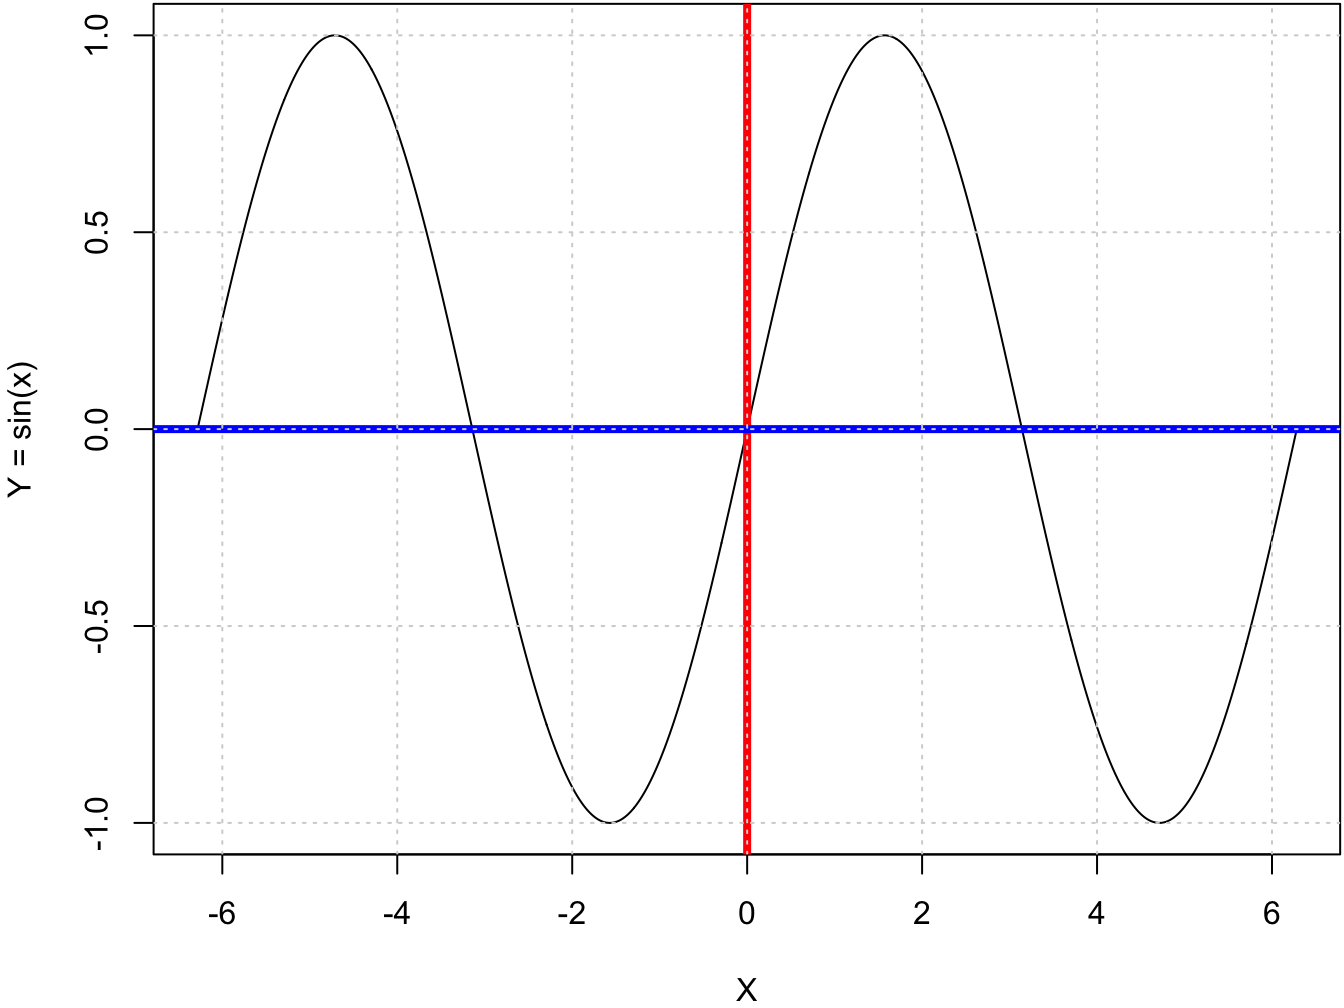
\includegraphics[width=0.8\linewidth]{R_in_Geoscience_files/figure-latex/fig.v1-1} 

}

\caption{R绘图结果}(\#fig:fig.v1)
\end{figure}

\begin{Shaded}
\begin{Highlighting}[]
\NormalTok{n=}\DecValTok{1000}
\NormalTok{x =}\StringTok{ }\DecValTok{1}\OperatorTok{:}\NormalTok{n}
\NormalTok{y =}\StringTok{ }\KeywordTok{abs}\NormalTok{(}\KeywordTok{rnorm}\NormalTok{(n, }\DataTypeTok{mean=}\DecValTok{10}\NormalTok{, }\DataTypeTok{sd=}\DecValTok{3}\NormalTok{))}
\NormalTok{y.sort =}\StringTok{ }\KeywordTok{sort}\NormalTok{(y)}
\KeywordTok{par}\NormalTok{(}\DataTypeTok{mfrow=}\KeywordTok{c}\NormalTok{(}\DecValTok{2}\NormalTok{,}\DecValTok{2}\NormalTok{))}
\KeywordTok{plot}\NormalTok{(x, y.sort, }\DataTypeTok{log=}\StringTok{\textquotesingle{}\textquotesingle{}}\NormalTok{); }\KeywordTok{grid}\NormalTok{()}
\KeywordTok{plot}\NormalTok{(x, y.sort, }\DataTypeTok{log=}\StringTok{\textquotesingle{}x\textquotesingle{}}\NormalTok{); }\KeywordTok{grid}\NormalTok{()}
\KeywordTok{plot}\NormalTok{(x, y.sort, }\DataTypeTok{log=}\StringTok{\textquotesingle{}y\textquotesingle{}}\NormalTok{); }\KeywordTok{grid}\NormalTok{()}
\KeywordTok{plot}\NormalTok{(x, y.sort, }\DataTypeTok{log=}\StringTok{\textquotesingle{}xy\textquotesingle{}}\NormalTok{); }\KeywordTok{grid}\NormalTok{()}
\end{Highlighting}
\end{Shaded}

\begin{figure}

{\centering 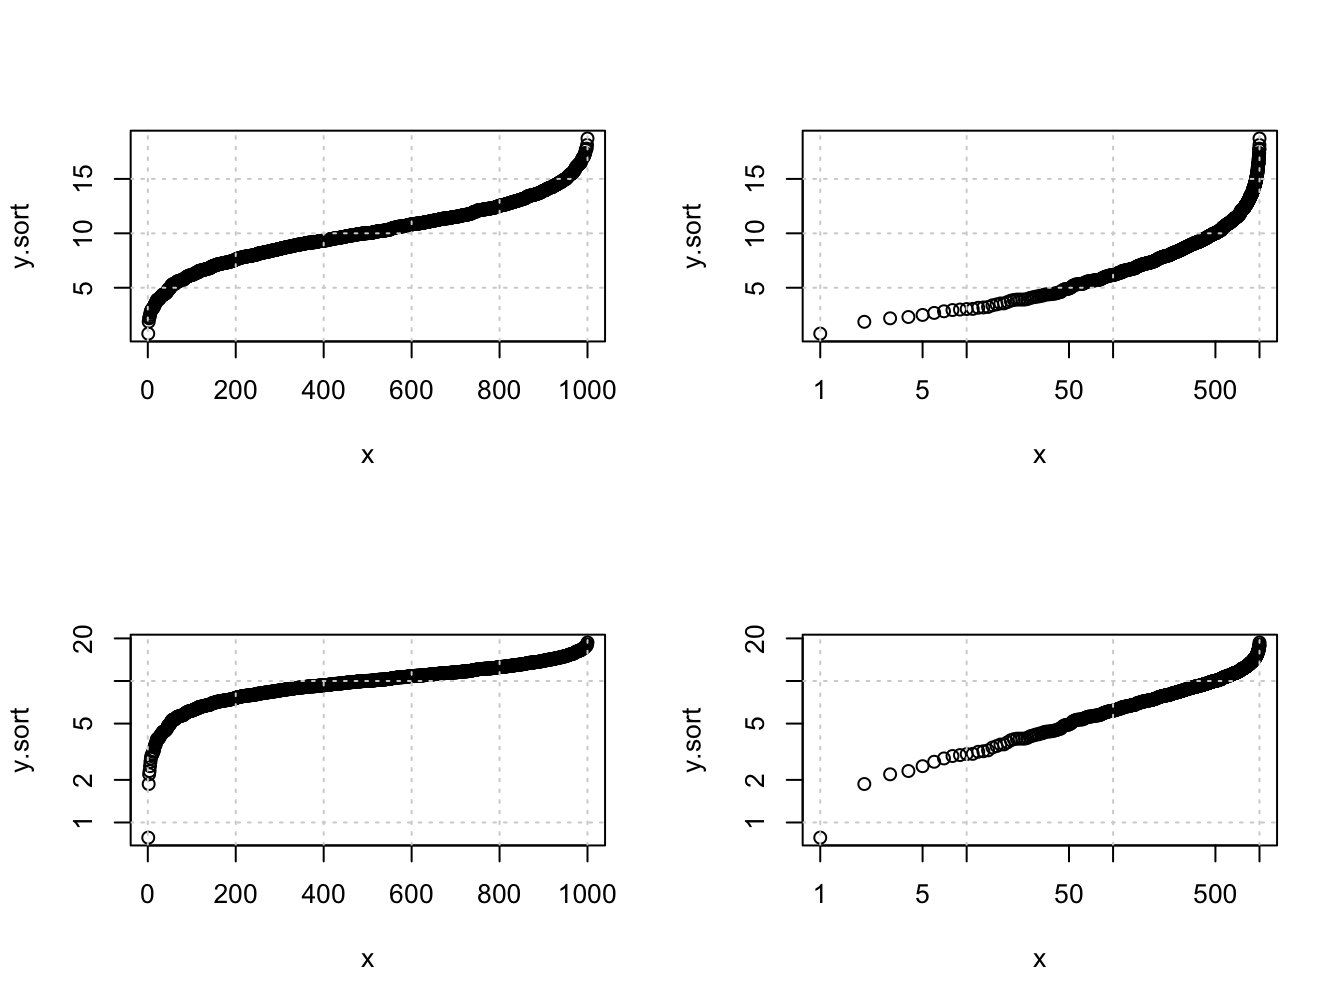
\includegraphics[width=0.8\linewidth]{R_in_Geoscience_files/figure-latex/unnamed-chunk-13-1} 

}

\caption{绘图:排序的随机数}\label{fig:unnamed-chunk-13}
\end{figure}

\hypertarget{ux4e09ux7ef4ux53efux89c6ux5316}{%
\section{三维可视化}\label{ux4e09ux7ef4ux53efux89c6ux5316}}

\begin{verbatim}
install.package('rgl')
\end{verbatim}

\begin{Shaded}
\begin{Highlighting}[]
\KeywordTok{library}\NormalTok{(rgl)}
\KeywordTok{with}\NormalTok{(iris, }\KeywordTok{plot3d}\NormalTok{(Sepal.Length, Sepal.Width, Petal.Length, }
                  \DataTypeTok{type=}\StringTok{"s"}\NormalTok{, }\DataTypeTok{col=}\KeywordTok{as.numeric}\NormalTok{(Species)))}
\end{Highlighting}
\end{Shaded}

\hypertarget{tsd}{%
\chapter{时间序列分析}\label{tsd}}

We describe our methods in this chapter.

\hypertarget{spatial}{%
\chapter{空间分析与可视化}\label{spatial}}

基本数据类型:矢量与栅格。

\begin{longtable}[]{@{}cc@{}}
\toprule
矢量数据 & 栅格数据\tabularnewline
\midrule
\endhead
数据存储量小 & 数据存储量大\tabularnewline
空间位置精度高 & 空间位置精度低\tabularnewline
用网络连接法能完整描述拓扑关系 & 难于建立网络连接关系\tabularnewline
输出简单容易,绘图细腻、精确、美观 & 输出速度快,但绘图粗糙、不美观\tabularnewline
可对图形及其属性进行检索、更新和综合 & 便于面状数据处\tabularnewline
数据结构复杂 & 数据结构简单\tabularnewline
获取数据慢 & 快速获取大量数据\tabularnewline
数学模拟困难 & 数学模拟方便\tabularnewline
多种地图叠合分析困难 & 多种地图叠合分析方便\tabularnewline
不能直接处理数字图像信息 & 能直接处理数字图像信息\tabularnewline
空间分析不容易实现 & 空间分析易于进行\tabularnewline
边界复杂、模糊的事物难以描述 & 容易描述边界复杂、模糊的事物\tabularnewline
数据输出的费用较高 & 技术开发费用低\tabularnewline
\bottomrule
\end{longtable}

\href{https://www.osgeo.cn/gis-tutorial/ch02/02_5.html}{矢量与栅格数据结构的比较}

\hypertarget{ux77e2ux91cfux6570ux636e}{%
\section{矢量数据}\label{ux77e2ux91cfux6570ux636e}}

\begin{itemize}
\tightlist
\item
  加载需要的库
\end{itemize}

\begin{Shaded}
\begin{Highlighting}[]
\KeywordTok{library}\NormalTok{(raster)  }\CommentTok{\#raster包用于绘图}
\KeywordTok{library}\NormalTok{(sp)  }\CommentTok{\#sp包用于矢量数据操作}
\KeywordTok{library}\NormalTok{(rgdal)  }\CommentTok{\# rgdal用于读写数据}
\KeywordTok{library}\NormalTok{(rgeos)  }\CommentTok{\# rgeos用于空间分析}
\end{Highlighting}
\end{Shaded}

\begin{itemize}
\item
  由坐标产生数据
\item
  读取数据
\end{itemize}

\begin{verbatim}
## OGR data source with driver: ESRI Shapefile 
## Source: "/Users/leleshu/Dropbox/workspace/Rwork/R_in_Geoscience/Excercise/Data_spatial/Province.shp", layer: "Province"
## with 924 features
## It has 7 fields
\end{verbatim}

\begin{verbatim}
## OGR data source with driver: ESRI Shapefile 
## Source: "/Users/leleshu/Dropbox/workspace/Rwork/R_in_Geoscience/Excercise/Data_spatial/City.shp", layer: "City"
## with 34 features
## It has 10 fields
\end{verbatim}

\begin{verbatim}
## OGR data source with driver: ESRI Shapefile 
## Source: "/Users/leleshu/Dropbox/workspace/Rwork/R_in_Geoscience/Excercise/Data_spatial/TibetPlateau.shp", layer: "TibetPlateau"
## with 1 features
## It has 1 fields
\end{verbatim}

\begin{figure}

{\centering 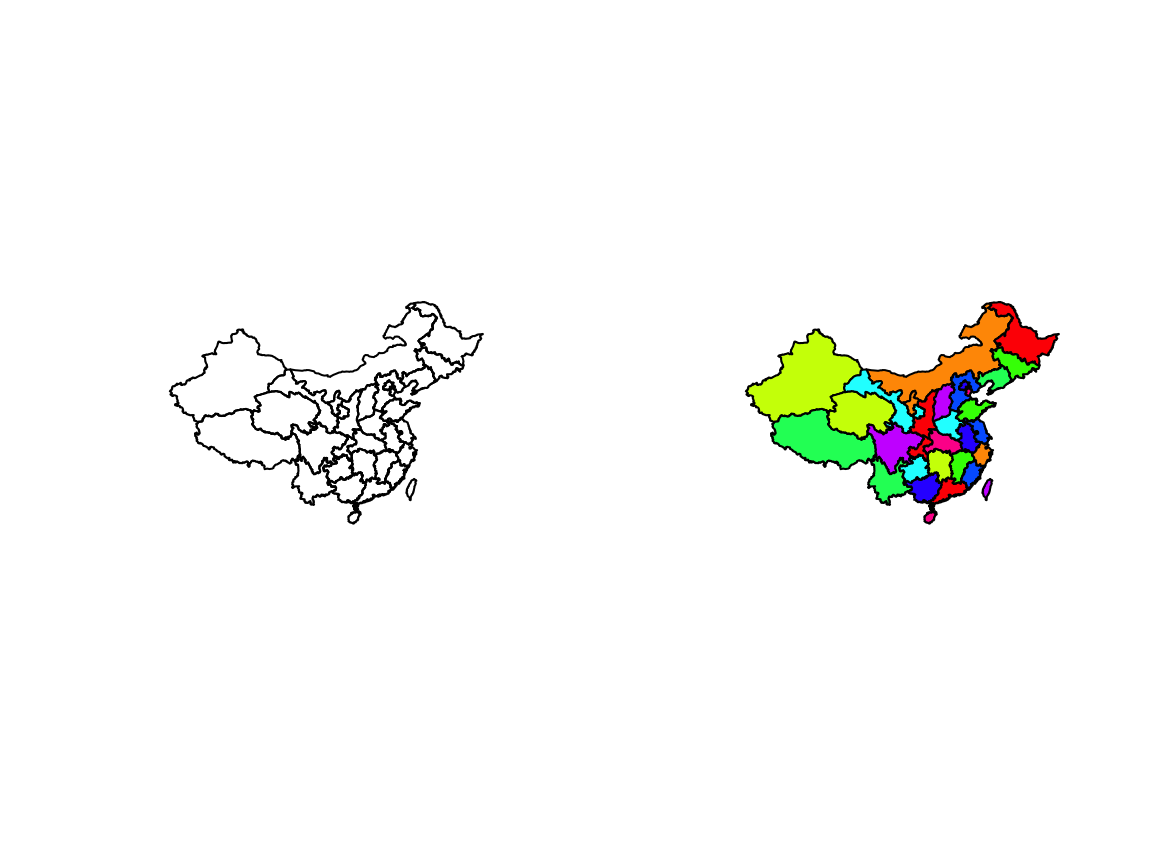
\includegraphics[width=0.8\linewidth]{R_in_Geoscience_files/figure-latex/ch4.read.sp-1} 

}

\caption{绘图:矢量地图}(\#fig:ch4.read.sp)
\end{figure}

\hypertarget{ai}{%
\chapter{机器学习}\label{ai}}

\hypertarget{ux673aux5668ux5b66ux4e60ux57faux7840}{%
\section{机器学习基础}\label{ux673aux5668ux5b66ux4e60ux57faux7840}}

\hypertarget{ux6570ux636eux5206ux7c7b}{%
\section{数据分类}\label{ux6570ux636eux5206ux7c7b}}

\hypertarget{ux65f6ux95f4ux5e8fux5217}{%
\section{时间序列}\label{ux65f6ux95f4ux5e8fux5217}}

\bibliography{book.bib,packages.bib}


\end{document}
